\documentclass[a4paper]{article}

\usepackage{mfirstuc}
\usepackage{graphicx}
\usepackage{amsmath}
\usepackage[fontsize=12pt]{scrextend}
\usepackage[bindingoffset=10mm,left=20mm,bottom=3cm]{geometry}
\usepackage{floatrow}
\usepackage{subfig}
\usepackage{hyperref}
\usepackage{array}
\floatsetup[figure]{capposition=bottom}
\floatsetup[table]{capposition=bottom}
\usepackage{amsfonts}
\floatplacement{figure}{H}
\floatplacement{table}{H}
\newcolumntype{P}[1]{>{\centering\arraybackslash}p{#1}}

\title{
  \pagenumbering{gobble}
  \vspace{-3cm}
  {\centering
\includegraphics[scale=0.1]{./img/logo}\par}
  \vspace{1cm}
  \centering
  {\scshape\LARGE Sapienza University of Rome \par}
  \vspace{1cm}
  {\Large\xcapitalisewords Faculty of {Information Engineering, Informatics and Statistics}\unskip\strut\par}
  \vspace{1cm}
  {\Large {Department of Computer, Control and Management Engineering (DIAG)}\unskip\strut\par}
  \vspace{2cm}
  {\scshape\Large Robotics2 Project\unskip\strut\par}
  {\scshape\Large Prof: Alessandro De Luca\unskip\strut\par}
  {\scshape\Large Tutor: Pietro Pustina\unskip\strut\par}
  \vspace{1.5cm}
  {\huge\bfseries\xcapitalisewords{D\lowercase{ata-driven identification \\of a one-link robot with flexible joint}}\unskip\strut\par}
  \vspace{2cm}
  {\Large\xcapitalisewords{Lorenzo Cirillo 1895955\\Claudio Schiavella 1884561}\unskip\strut\par}  
  \author{}
  \date{}
  \vfill
  {\large July 26, 2023\par}
}


\begin{document}

% ----------------------------------- Title ----------------------------------- %
\maketitle


% ---------------------------------- Contents --------------------------------- %
\pagenumbering{roman}
\tableofcontents


% ----------------------------------- Intro ----------------------------------- %
\pagenumbering{arabic}
\section{Introduction}
\label{sec:intro}
A manipulator robot can be described mathematically through its dynamic model. The latter illustrates the relationships between the generalized forces applied to the robot and the resulting motion of its mechanical structure. Various approaches exist to derive the model, such as D'Alembert's or Hamilton's principles. Specifically from the Hamiltonian approach are derived the Euler-Lagrange equations, used for modeling and control. This type of approach is energetic. It allows us to derive in symbolic form the equations of motion, enabling and encouraging the analysis of the dynamic properties of the robot and the possible controls to be applied to it. \\
In such a context, it is very easy to make a connection with neural networks. Indeed, the latter have demonstrated excellent capabilities in modeling systems over time, achieving very good performance and quality results. However, a generic neural network has difficulty generalizing to contexts in which conservation laws are present. Such a problem in the field of robotics is not good. \\
For this reason, \cite{lnncranmer} introduced a new type of neural network, called Lagrangian Neural Network (LNN), able to learn conservation laws\\
Our project uses both a baseline neural network and a LNN to learn the Lagrangian and consequently the dynamic model of single-link robots, with a rigid or elastic joint. The aim is to verify the functioning of the two methods, analyzing results and problems.
\\Consequently, the report will be structured as follows:
\begin{itemize}
    \item Section 2 introduces a parametric approach to the Euler-Lagrange equations based on Lagrangian functions, as proposed in \cite{lnncranmer}.

    \item Section 3 presents the dynamic models of the robots used in the simulations.
    
    \item Section 4 presents the architectures of the neural networks used in the simulations.

    \item Section 5 presents the settings and results of the simulations in various application contexts.
\end{itemize}


% ---------------------------- Parametric Lagrangian -------------------------- %
\section{Parametric Lagrangian}
\label{sec:parmlag}
The Lagrangian approach is based on a set of generalized coordinates $q\in\mathbb{R}^N$, where $n$ is the number of degrees of freedom of the robot. The Lagrangianis defined as difference between the kinetic energy $T(q,\dot{q})$ and the potential energy $U(q)$ of the system, i.e.

\begin{equation}
    \nonumber
    L(q,\dot{q}) = T(q,\dot{q}) - U(q).
\end{equation}

From this point we derive the Euler-Lagrange equations, assuming for our context the absence of dissipative forces

\begin{equation}
    \label{eq:eul_lag}
    \frac{d}{dt}\frac{\partial L}{\partial \dot{q}_i} - \frac{\partial L}{\partial q_i} = 0\qquad\textnormal{for} \quad i=1,...,N.
\end{equation}

Expanding \eqref{eq:eul_lag} for robotic systems, we obtain the well-known equation for manipulators

\begin{equation}
    \nonumber
    M(q)\ddot{q} + c(q,\dot{q}) + g(q) = 0.
\end{equation}

As suggested by the authors of \cite{lnncranmer}, the next step would be to find an analytical expression of the Lagrangian function and then expand the Euler-Lagrange equations to identify the dynamic model. However, this analytical form is not always known or easily obtained. Consequently, an alternative way is needed, which is proposed in \cite{lnncranmer}. Initially, it is necessary to rewrite \eqref{eq:eul_lag} in vector form  

\begin{equation}
    \nonumber
    \frac{d}{dt}\nabla_{\dot{q}} L = \nabla_{q} L.
\end{equation}

Next, we expand the time derivative across the gradient using the chain rule

\begin{equation}
    \nonumber
    (\nabla_{\dot{q}}\nabla_{\dot{q}}^T L)\ddot{q} + (\nabla_{q}\nabla_{\dot{q}}^T L)\dot{q} = \nabla_{q} L.
\end{equation}

At this point, with a simple matrix inversion, we obtain the expression of the acceleration vector

\begin{equation}
    \label{eq:paramlag3}
    \ddot{q} = (\nabla_{\dot{q}}\nabla_{\dot{q}}^T L)^{-1} [\nabla_{q} L - (\nabla_{q}\nabla_{\dot{q}}^T L)\dot{q}].
\end{equation}

The \eqref{eq:paramlag3} specializes in the \eqref{eq:paramlag4} when the system is a rigid robot.

\begin{equation}
    \label{eq:paramlag4}
    \ddot{q} = M(q)^{-1}[u - (c(q,\dot{q}) + g(q))].
\end{equation}

In conclusion, we can see how \eqref{eq:paramlag3} contains the Lagrangian to the right of the equal and its derivatives. By doing so, thanks to the automatic differentiation, learning the Lagrangian with a neural network we can calculate the acceleration. What is obtained can be fed into an integrator to find the entire dynamics of the system.


%------------------------------------- Robot ---------------------------------- %
\section{Robot}
\label{sec:robot}
In this section, dynamic models of the rigid and elastic 1R robots are derived for both the Euler Lagrange equations and the method proposed in \cite{lnncranmer}, as well as expressing these with state vectors so that they can be processed by integrators.

%---> Rigid Model
\subsection{Robot rigid model}
The model of a rigid robot is derived by assuming that the manipulator works in a vertical plane and that the $y$ axis of the frame is agreeing with the direction of gravity.\\
The kinetic energy is
\begin{equation}
    \nonumber
    T = \frac{1}{2}(I+md^2)\dot{q}^2,
\end{equation}
and consequently, the inertia matrix is
\begin{equation}
    M(q)=I+md^2.
\end{equation}
The Coriolis and centrifugal terms are computed in a classical way
\begin{equation}
    \nonumber
    C_1(q)=\frac{1}{2}(\frac{dM_1(q)}{dq}+(\frac{dM_1(q)}{dq})^T-\frac{dM(q)}{dq_1})=0
\end{equation}
\begin{equation}
    \nonumber
    c(q,\dot{q})=c_1(q,\dot{q})=\dot{q}^TC_1(q)\dot{q}=0
\end{equation}

We are not surprised by the zero value of $c(q,\dot{q})$. In fact, by having one single link, the centrifugal terms that contribute to the joint when it is moving are null. As a consequence, by having  $c(q,\dot{q})$ depends only on the single link of our robot, the result is canonical. \\

The potential energy is
\begin{equation}
    g=\begin{bmatrix}
        0 \\
        g_0 \\
        0
    \end{bmatrix},
\end{equation}
\begin{equation}
    U_g=-mg_0d\, \\cos(q),
\end{equation}
\begin{equation}
    g(q)=(\frac{dU_g}{dq})^T=mg_0d\, \sin(q),
\end{equation} \\

Consequently, the model is
\begin{equation}
\label{eq:rigid_model}
    (I+md^2)\ddot{q}+mg_0d\, \sin(q)=0.
\end{equation} \\

Finally, the acceleration obtained solving \eqref{eq:rigid_model} is
\begin{equation}
\label{eq:classical_rigid_acc}
    \ddot{q}=-\frac{1}{(I+md^2)}mg_0d\, \sin(q).
\end{equation}

\subsubsection{Parametric Lagrangian of rigid model}
Having computed the dynamic model from an analytical approach to the Lagrangian function, we can immediately make a comparison by observing the result that the application of the analytical Lagrangian function introduced in Section \ref{sec:parmlag}

\begin{equation}
    \label{eq:rig_eul_lag}
    L(q,\dot{q}) = T(q,\dot{q}) - U(q) = \frac{1}{2}(I+md^2)\dot{q}^2 + mg_0d\, \\cos(q) .
\end{equation}

From this Lagrangian expression, we derive all the elements needed to apply \eqref{eq:paramlag3}

\begin{equation}
    \nonumber
    \nabla_{\dot{q}}^{T} L = \frac{\partial L}{\partial \dot{q}} = (I+md^2)\dot{q}
\end{equation}

\begin{equation}
    \nonumber
    \nabla_{q} L = -mg_0d\,\sin(q)
\end{equation}

\begin{equation}
    \nonumber
    \nabla_{\dot{q}} \nabla_{\dot{q}}^{T} L = \frac{\partial^{2} L}{\partial \dot{q}^{2}} = (I+md^2)
\end{equation}

\begin{equation}
    \nonumber
    \nabla_{q} \nabla_{\dot{q}}^{T} L = \frac{\partial^{2} L}{\partial{q} \partial{\dot{q}}} = 0
\end{equation}

Thus obtaining a result that is shown to be equivalent to that found in equation \eqref{eq:classical_rigid_acc}, as expected
\begin{equation}
    \nonumber
    \ddot{q} = (\nabla_{\dot{q}}\nabla_{\dot{q}}^T L)^{-1} [\nabla_{q} L - (\nabla_{q}\nabla_{\dot{q}}^T L)\dot{q}] = -\frac{1}{(I+md^2)}mg_0d\, \sin(q).
\end{equation}

\subsubsection{Rigid state space}
Equation \ref{eq:rigid_model} can be expressed in state-space form by defining the $2\times1$ state vector

\begin{equation}
    \nonumber
    x = 
    \begin{bmatrix}    
        x_1 \\
        x_2 \\
    \end{bmatrix} = \begin{bmatrix}    
        q\\
        \dot{q}\\
    \end{bmatrix}.
\end{equation}

Accordingly, the dynamics of the system can be expressed as

\begin{equation}
    \nonumber
    \dot{x} = 
    \begin{bmatrix}    
        \dot{x}_1 \\
        \dot{x}_2 \\
    \end{bmatrix} = \begin{bmatrix}    
        x_2\\
        -\frac{1}{I+md^2}mg_0d\, \sin(q)\\
    \end{bmatrix}.
\end{equation}


%---> Elastic
\subsection{Robot elastic model}
Similar to the rigid case, we derive the dynamic model of the same robot, but with elasticity at the joint. In addition to the considerations made for the rigid robot, based also on what is expressed in \cite{sponge} and \cite{tomei}, we also assume that:

\begin{itemize}
    \item The coordinates frames of the motors are placed at their center of mass, as we understand the latter to be uniformly rotating bodies. The coordinate axes can thus be said to be principal axes, resulting in a diagonal inertia matrix.
    \item The kinetic energy of motors is mainly given by their rotation, so they will have a purely rotary motion.
    \item The motors are considered after the reduction ($\theta = \theta_m / n_r$). \\
\end{itemize}

The kinetic energy of the link ($T$) and motor($T_m$) are respectively:

\begin{equation}
    \nonumber
    T = \frac{1}{2} (I + md^2)\dot{q}^2 \qquad T_m = \frac{1}{2}, I_m \dot{\theta}^2.
\end{equation}

The inertia matrices for both cases are thus obtained

\begin{equation}
    \nonumber
    M(q) = I + md^2, \qquad B_m = I_m.
\end{equation}

As in the rigid case, it is immediate to see that the term of the Coriolis and Centrifugal forces turns out to be zero, due to the constant nature of the inertia matrix.

\begin{equation}
    \nonumber
    c(q,\dot{q}) = 0
\end{equation}

Finally, we derive the potential energies of the link and motor

\begin{equation}
    \nonumber
    U_m = 0, \qquad U_g = -mg_0d\, \cos(q), \qquad U_e = \frac{1}{2} k(q-\theta)^2 \dot{\theta},
\end{equation}
\begin{equation}
    \nonumber
    U = U_m + U_g + U_e = -mg_0d\, \cos(q) + \frac{1}{2}k(q-\theta)^2,
\end{equation}
\begin{equation}
    \nonumber
    g(q) = (\frac{\partial U}{\partial q})^T = mg_0d\, \sin(q) +k(q-\theta),\qquad (\frac{\partial U}{\partial \theta})^T = k(\theta - q) \dot{\theta}
\end{equation}

We thus obtain the dynamic model and the corresponding acceleration expressions
\begin{center}
\begin{equation}
    \nonumber
    \begin{cases}
        (I+md^2)\ddot{q}+mg_0d\, \sin(q) +k(q-\theta)=0\\
        I_m\ddot{\theta}+k(\theta-q)=0
    \end{cases}
\end{equation}
\begin{equation}
    \label{eq:el_mod9}
    \begin{cases}
        \ddot{q}=-\frac{1}{I+md^2}(mg_0d\, \sin(q)+k(q-\theta))\\
        \ddot{q}=\frac{1}{I_m}k(q-\theta)
    \end{cases}
\end{equation}
\end{center}

\subsubsection{Parametric Lagrangian of elastic model}
As we did in the rigid case, we can also see in the elastic context the result of applying the parametric Lagrangian function

\begin{equation}
    \nonumber
    L(q,\dot{q}) = T(q,\dot{q}) - U(q) = \frac{1}{2}(I+md^2)\dot{q}^2 + \frac{1}{2} I_m \dot{\theta}^2 + mg_0d\, \cos(q) - \frac{1}{2}\,k\,(q-\theta)^{2}.
\end{equation}

From this Lagrangian expression, we derive all the elements needed to apply equation \eqref{eq:paramlag3}

\begin{equation}
    \nonumber
    \nabla_{\dot{q}}^{T} L = 
    \begin{bmatrix}
        \frac{\partial L}{\partial \dot{q}} \\[3mm]
        \frac{\partial L}{\partial \dot{\theta}} \\
    \end{bmatrix} =
    \begin{bmatrix}
        (I+md^2)\dot{q}\\[1mm]
        I_m\dot{\theta}\\
    \end{bmatrix},
\end{equation}

\begin{equation}
    \nonumber
    \nabla_{\dot{q}}^{T} L = 
    \begin{bmatrix}
        \frac{\partial L}{\partial q} \\[3mm]
        \frac{\partial L}{\partial \theta} \\
    \end{bmatrix} =
    \begin{bmatrix}
        -mg_0d\,\sin(q) - k(q-\theta) \\
        k(q-\theta)\\
    \end{bmatrix},
\end{equation}

\begin{equation}
    \nonumber
    \nabla_{\dot{q}} \nabla_{\dot{q}}^{T} L =
    \begin{bmatrix}
        \frac{\partial L^2}{\partial \dot{q}^2} & \frac{\partial L^2}{\partial \dot{\theta} \partial \dot{q}} \\
        \frac{\partial L^2}{\partial \dot{q} \partial \dot{\theta}} & \frac{\partial L^2}{\partial \dot{\theta}^2} \\
    \end{bmatrix} =
    \begin{bmatrix}
        I+md^2 & 0 \\
        0 & I_m \\
    \end{bmatrix},
\end{equation}

\begin{equation}
    \nonumber
    \nabla_{q} \nabla_{\dot{q}}^{T} L =
    \begin{bmatrix}
        \frac{\partial L^2}{\partial \dot{q}^2} & \frac{\partial L^2}{\partial \theta \partial \dot{q}} \\
        \frac{\partial L^2}{\partial q \partial \dot{\theta}} & \frac{\partial L^2}{\partial \dot{\theta}^2} \\
    \end{bmatrix} =
    \begin{bmatrix}
        0 & 0 \\
        0 & 0 \\
    \end{bmatrix}.
\end{equation}


thus obtaining

\begin{equation}
    \label{eq:rig_eul_lag_7}
    \begin{bmatrix}    
        \ddot{q} \\
        \ddot{\theta}
    \end{bmatrix} = (\nabla_{\dot{q}}\nabla_{\dot{q}}^T L)^{-1} [\nabla_{q} L - (\nabla_{q}\nabla_{\dot{q}}^T L)\dot{q}] =
    \begin{bmatrix}
        -\frac{1}{I+md^2} (mg_0d\, \sin(q) + k(q-\theta)\\
        \frac{1}{I_m} k(q-\theta)
    \end{bmatrix}.
\end{equation}
\subsubsection{Elastic state space}
Equation shown in \ref{eq:el_mod9} can be expressed in state-space form by defining the $4\times1$ state vector

\begin{equation}
    \nonumber
    x = 
    \begin{bmatrix}    
        x_1 \\
        x_2 \\
        x_3 \\
        x_4 \\
    \end{bmatrix} = \begin{bmatrix}    
        q\\
        \theta\\
        \dot{q}\\
        \dot{\theta}\\
    \end{bmatrix}.
\end{equation}

Accordingly, the dynamics of the system can be expressed as

\begin{equation}
    \nonumber
    \dot{x} = 
    \begin{bmatrix}    
        \dot{x}_1 \\
        \dot{x}_2 \\
        \dot{x}_3 \\
        \dot{x}_4 \\
    \end{bmatrix} = \begin{bmatrix}    
        x_3\\
        x_4\\
        -\frac{1}{I+md^2} (mg_0d\, \sin(q) + k(q-\theta))\\
        \frac{1}{I_m} k(q-\theta)\\
    \end{bmatrix}
\end{equation}


%-------------------------------- NN architectures ---------------------------- %
\section{Neural Network Architectures}
\label{sec:nn_arch}
This section describes the two architectures that will be the subject of our simulations, one classical and one LNN. In particular, the approach that each network has toward the problem of robot dynamics estimation will be analyzed in depth.
%---> Baseline
\subsection{Baseline Neural Network}
\begin{figure}
\begin{center}
    \label{img:baseline_arch}
    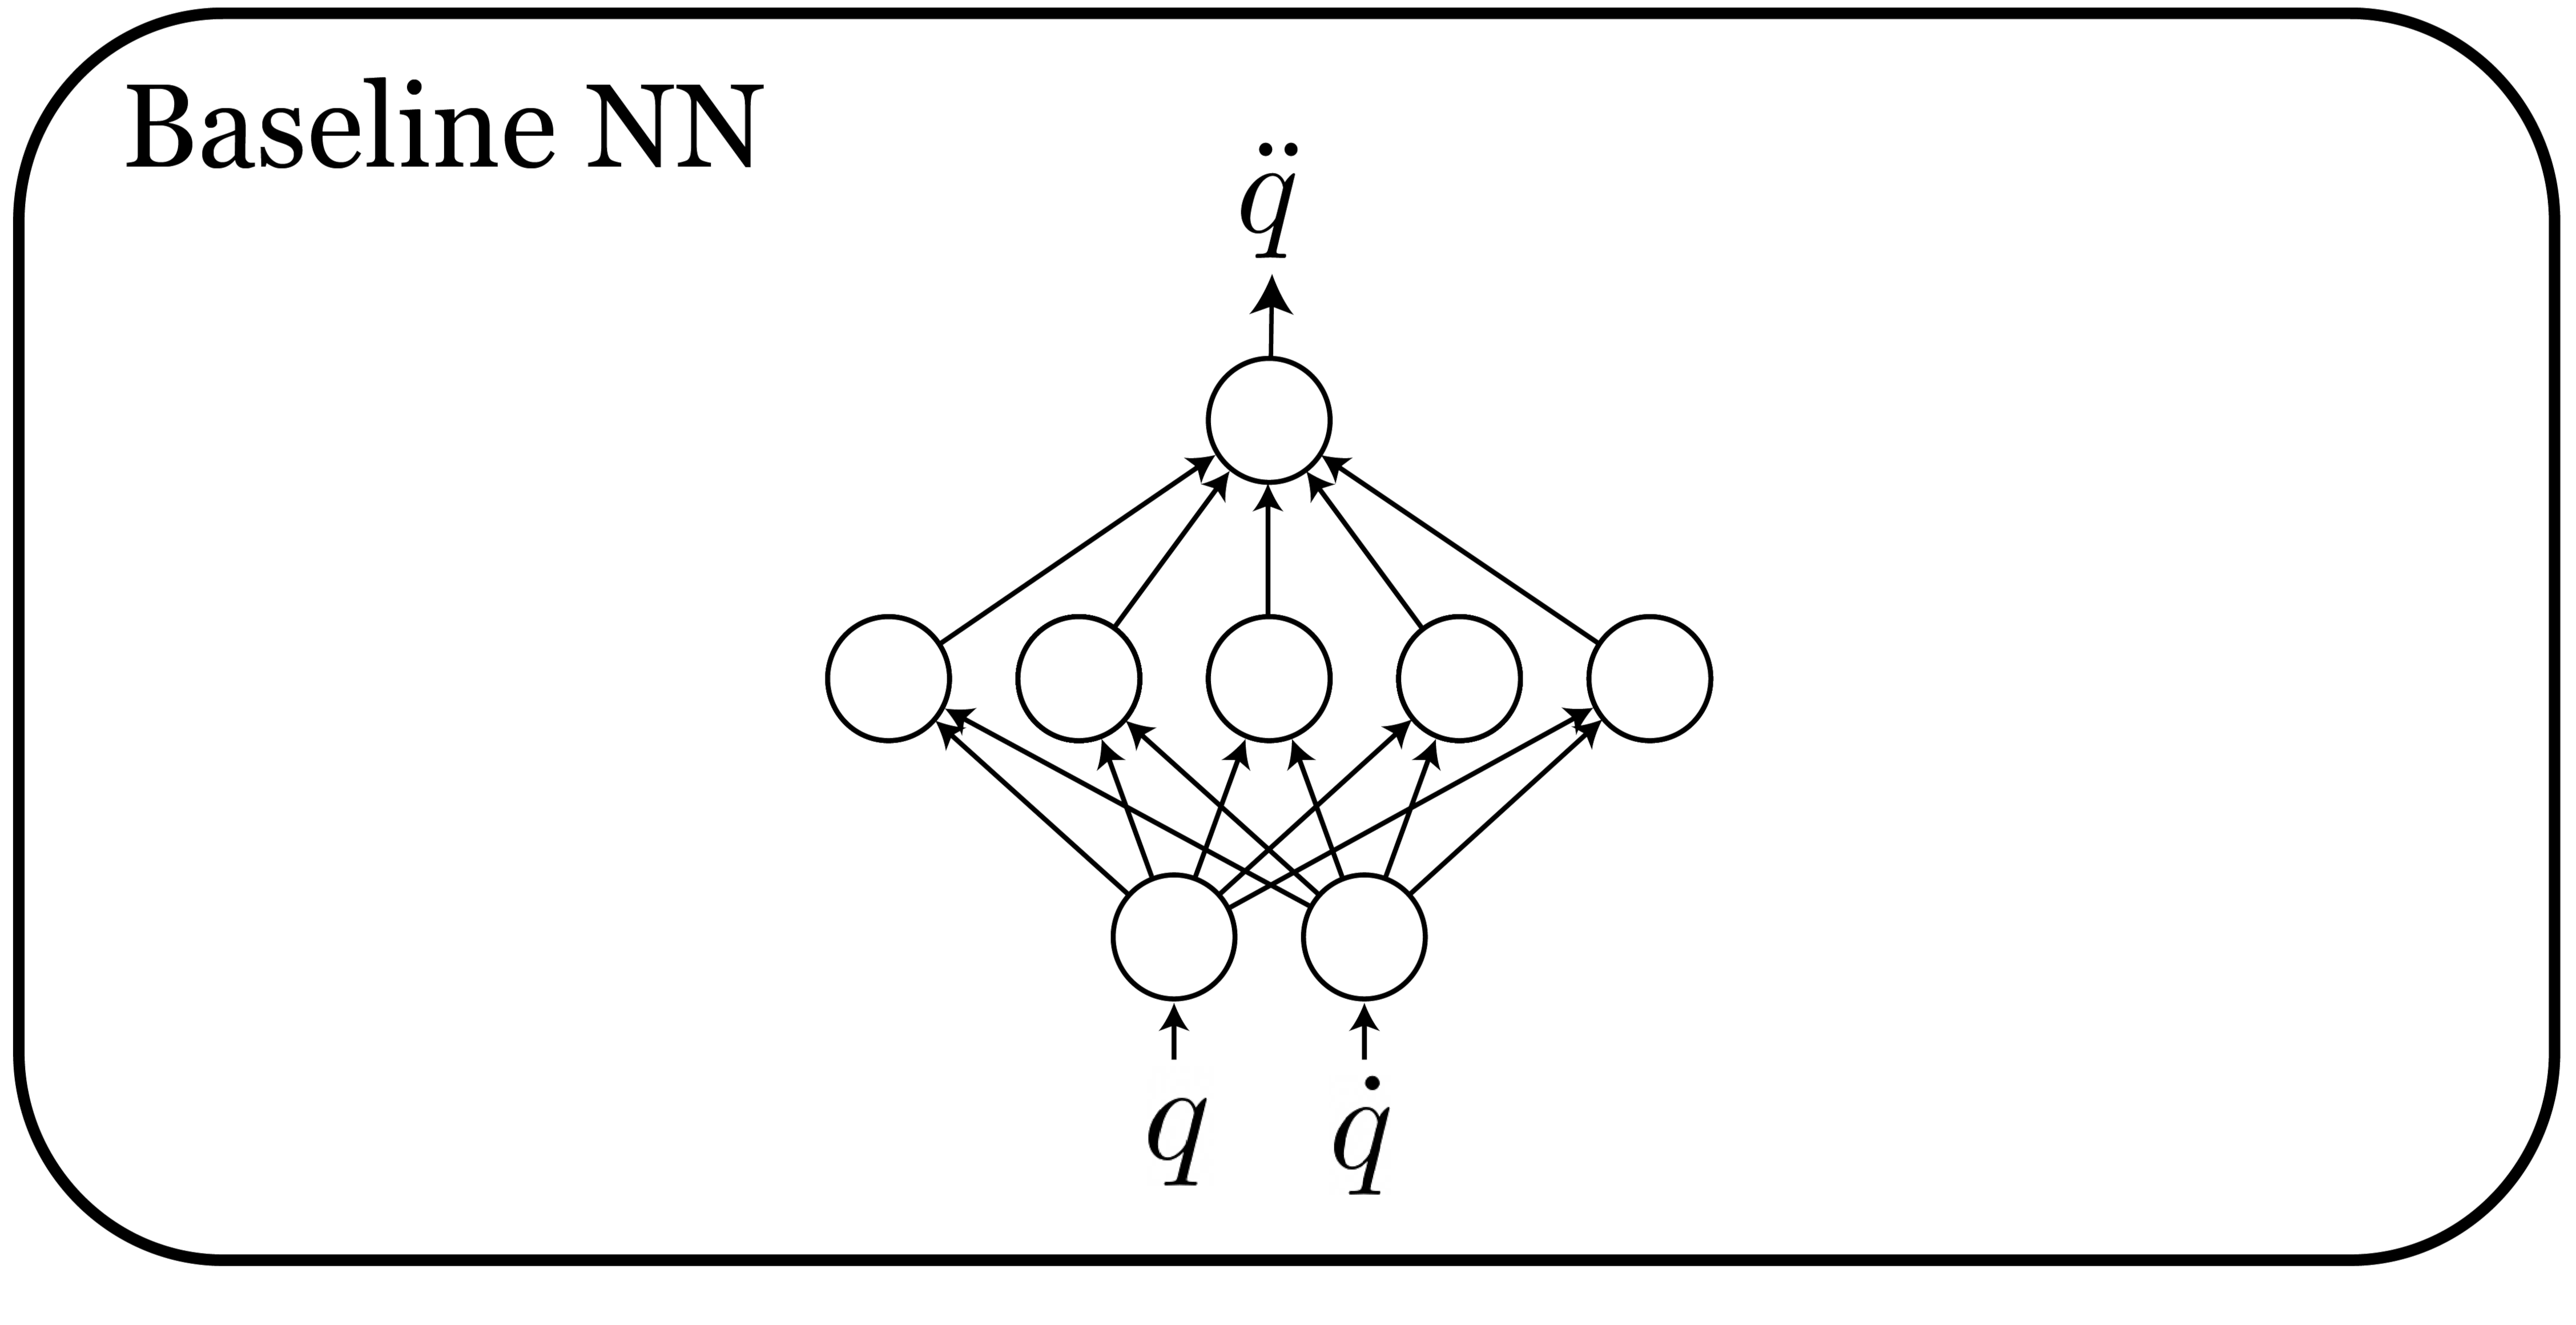
\includegraphics[scale=0.1]{./img/baseline_nn.png}  
    \caption{Baseline NN architecture}
\end{center}
\end{figure}

The first architecture we consider is a classical feedforward neural network, consisting only of fully connected layers.\\ This network tries to learn the acceleration $\ddot{q}$ directly from the configuration $q$ and the velocity $\dot{q}$, but without considering the Lagrangian and the constraints imposed by it via \eqref{eq:paramlag3}.\\ We use this network as a baseline against which to compare the LNN approach to the problem.\\ As for the various activation functions and other network parameters such as the number of layers and the number of neurons, we use the same as those of the LNN, to strengthen the comparison with the baseline.

%---> Lagrangian Neural Network
\subsection{Lagrangian Neural Network}
\begin{figure}
\begin{center}
    \label{img:lnn_arch}
    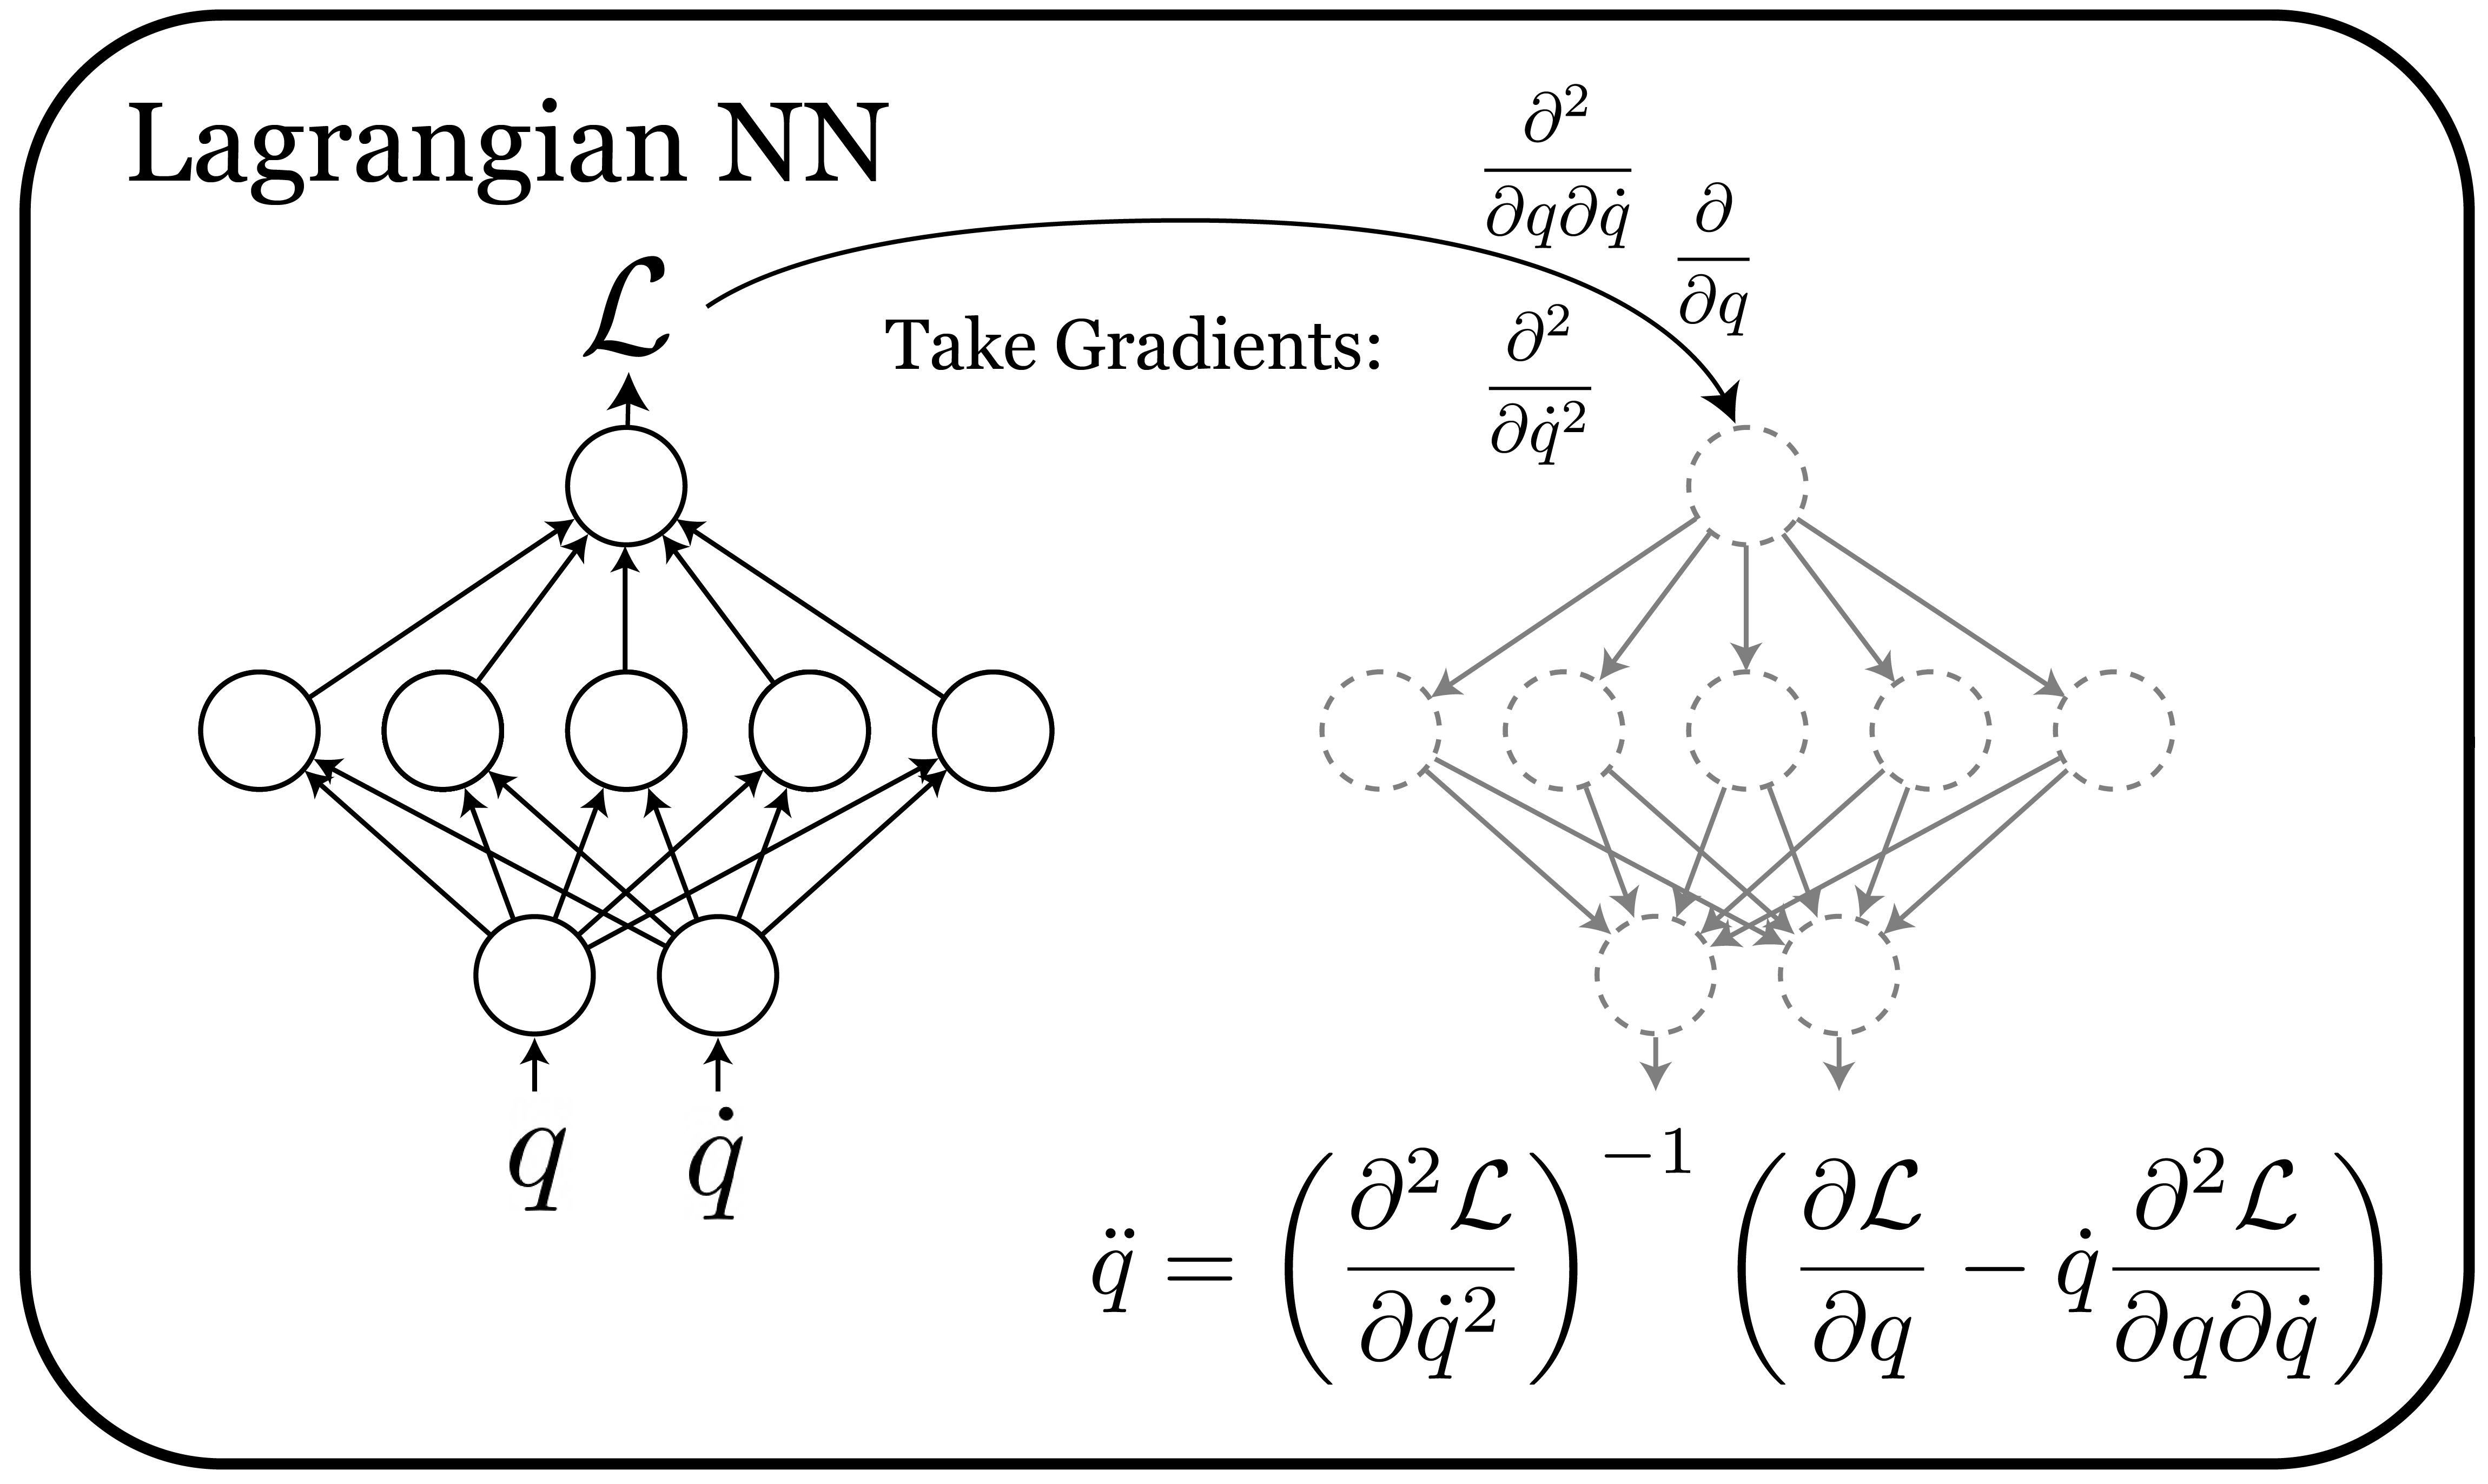
\includegraphics[scale=0.1]{./img/lnn.png}  
    \caption{LNN architecture}
\end{center}
\end{figure}
At least structurally, the LNN turns out to be very similar, if not the same, as the structure of the baseline NN. However, the approach by which prediction is arrived at is completely overturned. In fact, in this case, the goal of the LNN is to predict, or rather model, the parametric Lagrangian function, in a functional programming context. This approach is completely different from that applied by the baseline NN, which, aims immediately to predict the value of the acceleration given the position and velocity inputs. In the case of the LNN we can see that once the parametric Lagrangian function is obtained, the gradients are applied as shown in Section \ref{sec:parmlag}. Only after this process, the acceleration is obtained and compared with its ground truth. We can immediately conclude that this process is much closer to the nature of the robot than the baseline NN approach. The acceleration comes from a Lagrangian function, even if a black box of a parametric nature. By doing so, the prediction will benefit all the features, or at least the learned features, that a Lagrangian approach has.

%---------------------------------- Simulations ------------------------------- %
\section{Simulations}
\label{sec:sim}
In this section, we present the simulations carried out to observe the behavior of the two neural network architectures presented in Section \ref{sec:nn_arch} on the robot models obtained in Section \ref{sec:robot} and compare their results. The first type of simulation is based on observing the behavior of the networks in replicating the robot's dynamics. The second type, on the other hand, presents the same task but with the presence of noise to highlight how robust these architectures are in non-optimal contexts. Both types of tests will compare the true trajectory with the one calculated from the baseline NN and LNN, also showing the error between the ground truth and predictions and highlighting the Root Mean Square Error (RMSE) of the two cases \\
\begin{equation}
    \nonumber
    \text{RMSE}(y, \hat{y}) = \sqrt{\frac{\sum_{i=0}^{N - 1} (y_i - \hat{y}_i)^2}{N}}
\end{equation}

where $y$ is the ground truth, $\hat{y}$ are the predictions and $N$ is
the size of the data.

The above approach will be observed on various types of trajectories and for the elastic case, the evolution of the motor configuration will of course also be taken into account. There will be also a focus on how the networks manage to conserve the total energy of the system. The time steps in the graphs are intended to be in tenths of seconds, as proposed in \cite{lnncranmer}.

%---> Dataset generation
\subsection{Dataset generation}
Starting from 300 initial conditions, based on the equations obtained from Section \ref{sec:robot}, trajectories were derived over a time interval of 100-time steps with which to compose the dataset. The latter were obtained by the application of the differential equation solver odeint, on the previously exposed data. The entire available dataset is divided into train data and test data, as in the standard neural network training approach. Specifically, train data is $70\%$ and validation data is $30\%$ of the total. Following training, simulations are performed on trajectories generated ad-hoc for the test.

%---> Networks setup
\subsection{Rigid case}
\label{sub:rig_sims}
The choice of the values to assign to the robot parameters is very important since, if they are inconsistent, the obtained results can be flawed and not truthful. Rigid robot parameters are:
\begin{itemize}
    \item Link length ($l$).
    \item Link base radius ($r$).
    \item Link CoM distance from the base ($d$).
    \item Link mass ($m$).
    \item Link inertia ($I$).
\end{itemize}

Let us assume that the only link of the rigid robot we are analyzing: 
\begin{itemize}
    \item It is a tall aluminum cylinder.
    \item Its mass is uniformly distributed.
    \item Its density is $D_{all}=2700 \frac{kg}{m^3}$.
    \item Its inertia is mainly given by its length $l$.
\end{itemize} 
At this point, we can derive its mass and inertia from the following formulas
\begin{equation}
    \label{eq:cilinder}
    m=D_{all}V, \qquad  V=lr^2\pi, \qquad    I=\frac{1}{2}ml^2.
\end{equation}

After these considerations, we can define the parameters of the rigid robot that we will use in the simulations

\begin{table}
\centering
\caption{Rigid robot parameters}
\begin{tabular}{P{2.5cm}P{2.5cm}} 
\hline\hline
 \textbf{Parameter} & \textbf{Measure} \\ 
\hline
 Length & $0.30\, [m]$\\ 
\hline
 Base radius & $0.01\, [m]$\\ 
\hline
 CoM distance & $0.15\, [m]$\\ 
\hline
 Mass & $0.25\, [kg]$\\
\hline
 Inertia & $0.01125\, [kg\,m^2]$\\
\hline\hline
\end{tabular}
\end{table}

\subsubsection{Network setup}
\label{sub:rigid_train}
As anticipated in Section \ref{sec:nn_arch} both networks were set with the same structural parameters. In particular, the following values were chosen: 4 layers, 500 neurons, and Softplus activation function.

In addition, the train of both networks was set for several epochs equal to 10000 and a Mean Absolute Error (MAE) loss, as implemented in \cite{lnncranmer}.

\begin{equation}
    \nonumber
    \text{MAE}(y, \hat{y}) = \frac{ \sum_{i=0}^{N - 1} |y_i - \hat{y}_i| }{N}
\end{equation}

In the previous equation $y$ is the ground truth, $\hat{y}$ are the predictions and $N$ is the size of the past batch of data.\\

It should be mentioned that the loss has a regularisation mechanism, adding an L2 penalty term to the MSE value to avoid overfitting.
The optimizer used is Adam, which applied an adaptive learning rate to increase the effectiveness of the training. Additionally, the update of weights occurred only in particular contexts, such as reaching a threshold of epochs or improving loss. This approach, also recommended in \cite{lnncranmer} aims to optimize training time.
%---> Rigid Results
\subsubsection{Results}
First, we report the graphics of the test and train losses for the baseline NN and the LNN in \ref{fig:rigid_losses}:

\begin{figure}
    \centering
    \subfloat[\centering Baseline NN]{{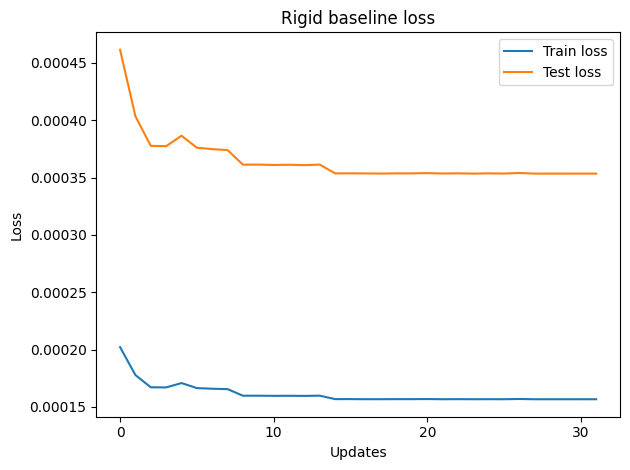
\includegraphics[width=6cm]{img/final_results/rigid/loss/Rigid_baseline_loss.png} }}
    \qquad
    \subfloat[\centering LNN]{{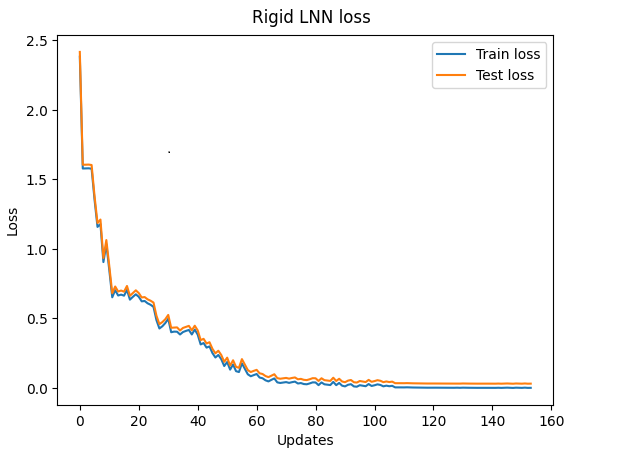
\includegraphics[width=6.5cm]{img/final_results/rigid/loss/rigid_lnn_loss.png} }}
    \caption{Test and train losses}
    \label{fig:rigid_losses}
\end{figure}

As we can see in figure \ref{fig:rigid_losses}, both the test and the train losses decrease for the baseline and the LNN. Anyway, we can see that the LNN has more consistent learning than the baseline NN because of the much more pronounced decrease in loss.\\ However, to confirm our intuitions, it is necessary to proceed with testing. After the training phase, we experimented with trained models of both networks on about ten different trajectories. We report the most significant results next.\\

\textbf{Simulation 1:} \textbf{Trajectory with $q(0)=1.33\, rad$, $\dot{q}(0)=0.2\, \frac{rad}{s}$}
In the first simulation, we compare the behavior of the two networks for the following desired trajectory

\begin{figure}
    \centering
    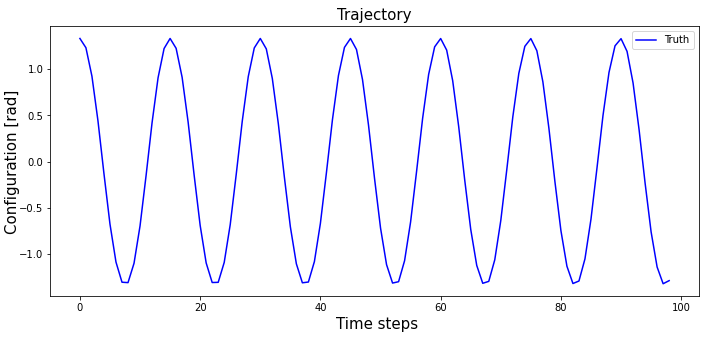
\includegraphics[scale=0.7]{img/final_results/rigid/76deg_02rads/traj_76_02.png}
    \caption{\textit{Simulation 1}. Plot of the desired trajectory for initial conditions $q(0)=1.33\, rad$, $\dot{q}(0)=0.2\, \frac{rad}{s}$}
    \label{fig:desired_rigid_76degrees_02rads}
\end{figure}

\begin{figure}
    \centering
    \subfloat[\centering Without noise \label{fig:rigid_76degrees_02rads_a}]{{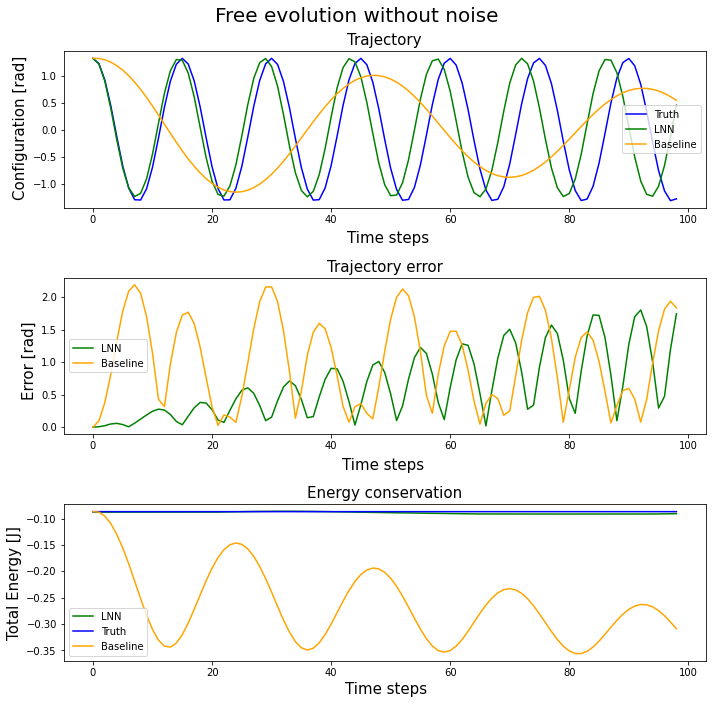
\includegraphics[width=6.5cm]{img/final_results/rigid/76deg_02rads/rigid_baseline_noisefree_76_02.png} }}
    \qquad
    \subfloat[\centering With noise \label{fig:rigid_76degrees_02rads_b}]{{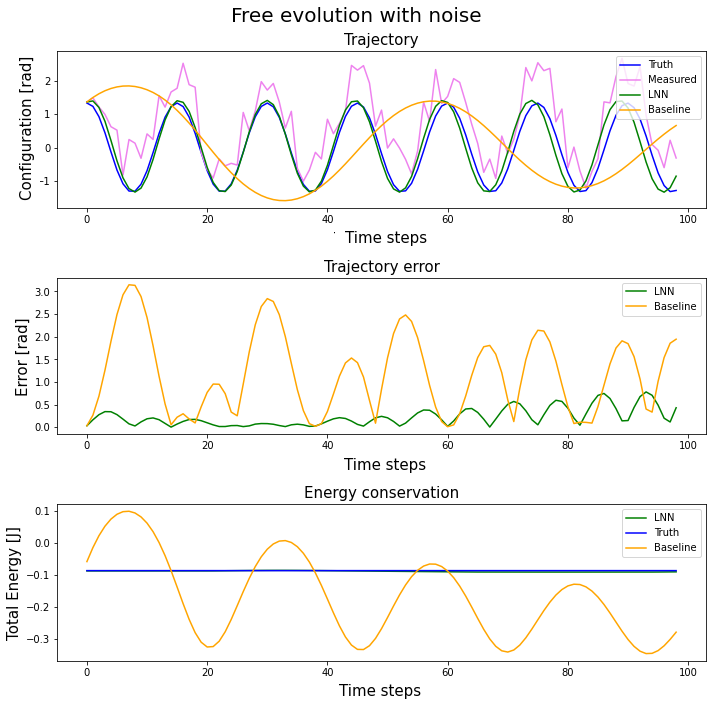
\includegraphics[width=6.5cm ]{img/final_results/rigid/76deg_02rads/rigid_baseline_noise_76_02.png} }}
    \caption{\textit{Simulation 1}. Graphs of the trajectory, error, and energy conservation for the NN baseline and LNN. The LNN approach demonstrates better results than the NN baseline.}
    \label{fig:rigid_76degrees_02rads}
\end{figure}

As we can see from figure \ref{fig:rigid_76degrees_02rads_a}, very good behavior of the LNN in both study cases is evident. Starting with the noiseless context, it can be seen that, especially at the initial moments of the trajectory, the LNN returns values that are almost coincident with the true trajectory, however, gaining an advance as time passes. The baseline NN, on the other hand, while guessing at least the sinusoidal trend of the trajectory, is certainly much less correct. Based on what was presented in Section \ref{sec:intro}, it turns out to be of interest to observe the conservation of total energy. Here we can see how the LNN achieves a very good result, completely overlapping the ground truth and, consequently, indicating full conservation of total energy.  This behavior is not present in the baseline NN, as expected. 

\begin{table}
    \centering
    \caption{\textit{Simulation 1.} LNN and baseline NN RMSE on the whole desired trajectory for initial conditions $q(0)=1.33\, rad$, $\dot{q}(0)=0.2\, \frac{rad}{s}$}
    \begin{tabular}{P{2.5cm}P{2.5cm}P{2.5cm}} 
    \hline\hline
    \textbf{Network} & \textbf{No noise} & \textbf{Noise} \\ 
    \hline
     Baseline NN & $1.2141\, [rad]$ & $1.4715\, [rad]$\\
    \hline
     LNN & $0.8175\, [rad]$& $0.2980\, [rad]$\\
    \hline\hline
    \end{tabular}
    \label{tab:rigid_rmse_1}    
\end{table}

So far we have been able to see how, under ideal conditions, we can confirm what we have deduced theoretically. However, to verify the actual robustness of the proposed architectures, we can see in figure \ref{fig:rigid_76degrees_02rads_b} how the latter react when the data from which they are to predict the trajectory are subjected to uniform noise, which pollutes the measurement with random samples between $\pm \frac{\pi}{2}$.
We can see that the trend we had in the case without noise is also maintained in the case with noise. The LNN succeeds very well in predicting the trajectory, even at the time when the data is plagued by noise. In this case, moreover, the lag behavior as time passes seems to be less consistent, which is also confirmed by the results in table \ref{tab:rigid_rmse_1} that show a lower RMSE of the LNN in the noisy case than in the clean case. The goodness of the LNN results is also confirmed in the context of energy conservation. For the baseline NN, the noisy case introduces additional difficulties for this approach, which tends to worsen its results.\\

\textbf{Simulation 2:} \textbf{Trajectory with $q(0)=0\, rad$, $\dot{q}(0)=4\, \frac{rad}{s}$}
We now observe how the two architectures can react at a level of initial speed that is certainly much higher than the previous

\begin{figure}
    \centering
    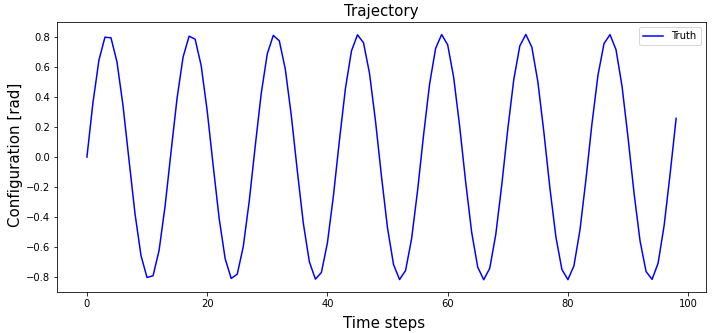
\includegraphics[scale=0.7]{img/final_results/rigid/0deg_4rads/traj_0_4.png}
    \caption{\textit{Simulation 2}. Plot of the desired trajectory for initial conditions $q(0)=0\, rad$, $\dot{q}(0)=4\, \frac{rad}{s}$}
    \label{fig:desired_rigid_0degrees_4rads}
\end{figure}

\begin{figure}
    \centering
    \subfloat[\centering Without noise \label{fig:rigid_0degrees_4rads_a}]{{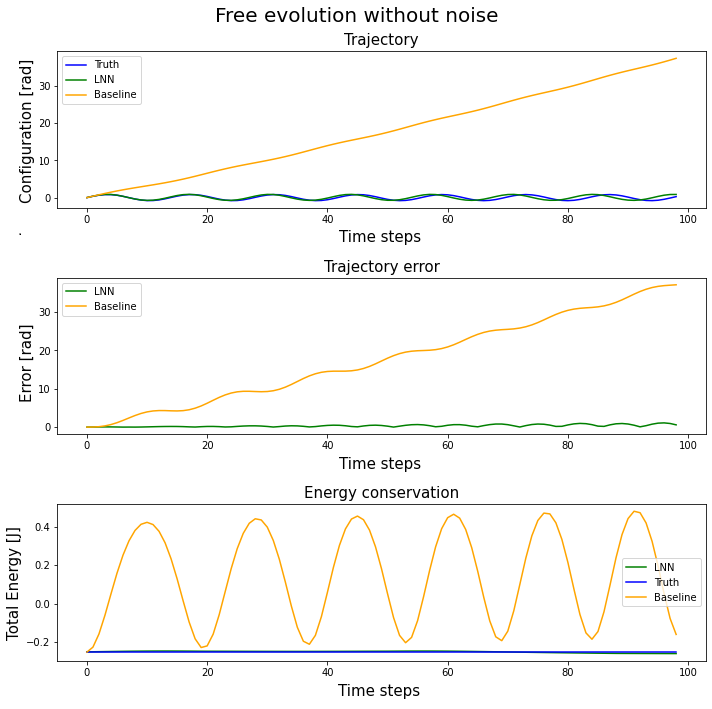
\includegraphics[width=6.5cm]{img/final_results/rigid/0deg_4rads/rigid_baseline_noisefree_0_4.png} }}
    \qquad
    \subfloat[\centering With noise \label{fig:rigid_0degrees_4rads_b}]{{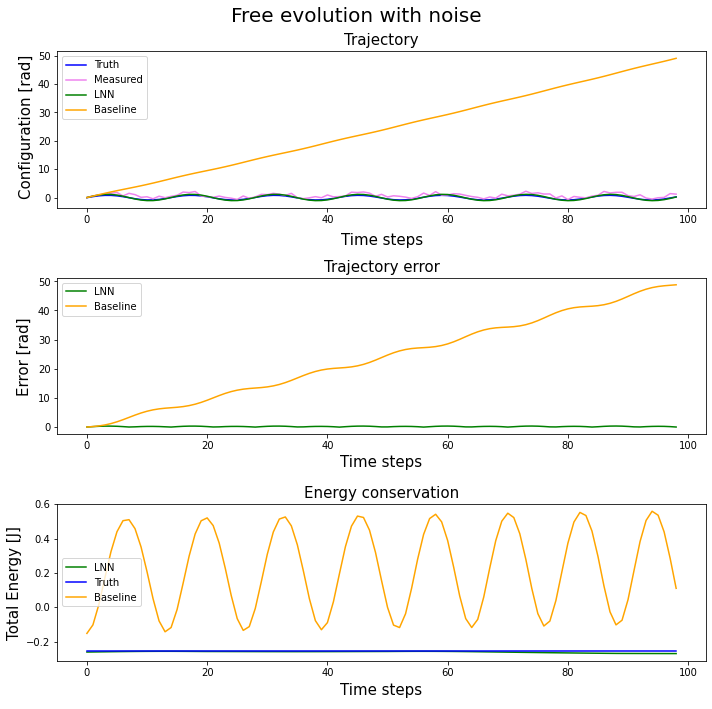
\includegraphics[width=6.5cm ]{img/final_results/rigid/0deg_4rads/rigid_baseline_noise_0_4.png} }}
    \caption{\textit{Simulation 2}. Graphs of the trajectory, error, and energy conservation for the NN baseline and LNN. For these initial conditions, the baseline NN demonstrates anomalous behavior, while the LNN continues to demonstrate very good properties in application contexts.}
    \label{fig:rigid_0degrees_4rads}
\end{figure}

The first thing that is highlighted by all the graphs in figure \ref{fig:rigid_0degrees_4rads} is how in both scenarios of the simulation, without noise and with, the NN baseline acquires a strongly abnormal behavior, returning a trajectory that has very little good, if any, to it. On the other hand, looking at the LNN results, the difference in performance is obvious and remarkable. Above all, it is interesting to note that LNN again maintains very good total energy conservation behavior.\\

\begin{table}
    \centering
    \caption{\textit{Simulation 2.} LNN and baseline NN RMSE on the whole desired trajectory for initial conditions $q(0)=0\, rad$, $\dot{q}(0)=4\, \frac{rad}{s}$}
    \begin{tabular}{P{2.5cm}P{2.5cm}P{2.5cm}} 
    \hline\hline
    \textbf{Network} & \textbf{No noise} & \textbf{Noise} \\ 
    \hline
     Baseline NN & $20.8874\, [rad]$ & $28.0418\, [rad]$\\
    \hline
     LNN & $0.4576\, [rad]$& $0.2227\, [rad]$\\
    \hline\hline
    \end{tabular}
    \label{tab:rigid_rmse_2}    
\end{table}

Also from the RMSE results in table \ref{tab:rigid_rmse_2}, the LNN performs very accurately in both the normal and noisy contexts. Compared with the results of \textit{Simulation 1} we see that for LNN the RMSE index is lower in both study cases. Most likely this is to be associated with the fact that the advance of the trajectory predicted by the LNN occurs later in the execution time.\\

\textbf{Simulation 3:} \textbf{Trajectory with $q(0)=2.66\, rad$, $\dot{q}(0)=0.5\, \frac{rad}{s}$} To conclude our simulations on the rigid case, we decide to try a trajectory in which the robot starts from a much more pronounced position than the previous ones, positioning it almost mirroring its position at $0 rad$

\begin{figure}
    \centering
    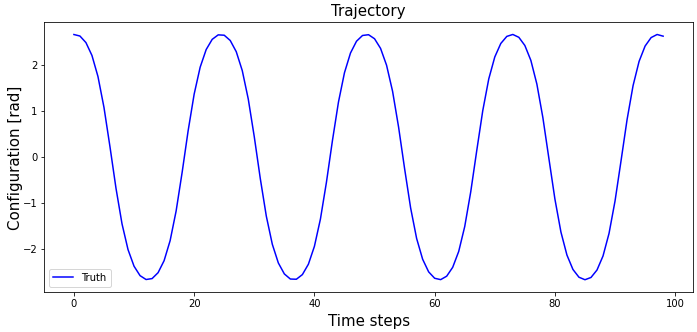
\includegraphics[scale=0.7]{img/final_results/rigid/150deg_05rads/traj_150_05.png}
    \caption{\textit{Simulation 2}. Plot of the desired trajectory for initial conditions $q(0)=2.66\, rad$, $\dot{q}(0)=0.5\, \frac{rad}{s}$}
    \label{fig:desired_rigid_150degrees_05rads}
\end{figure}

\begin{figure}
    \centering
    \subfloat[\centering Without noise \label{fig:rigid_150degrees_05rads_a}]{{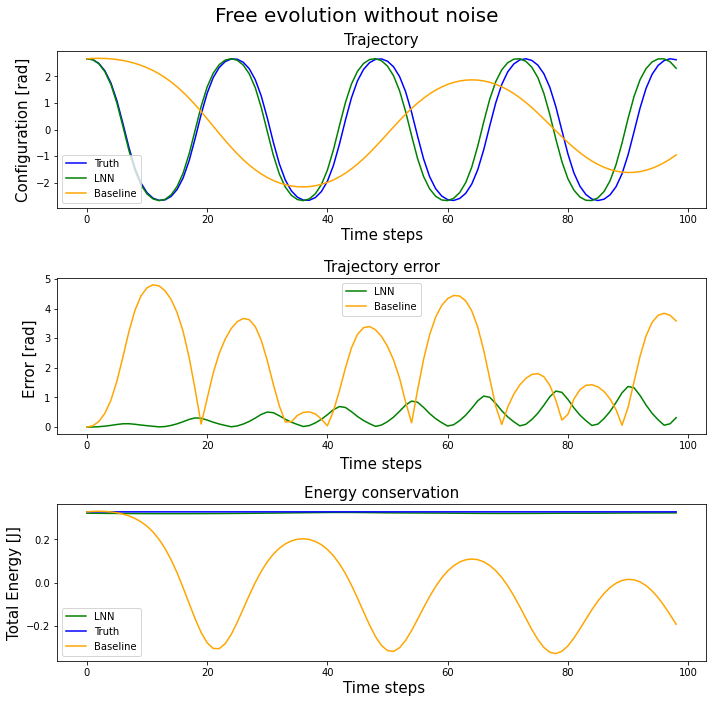
\includegraphics[width=6.5cm]{img/final_results/rigid/150deg_05rads/rigid_baseline_noisefree_150_05.png} }}
    \qquad
    \subfloat[\centering With noise \label{fig:rigid_150degrees_05rads_b}]{{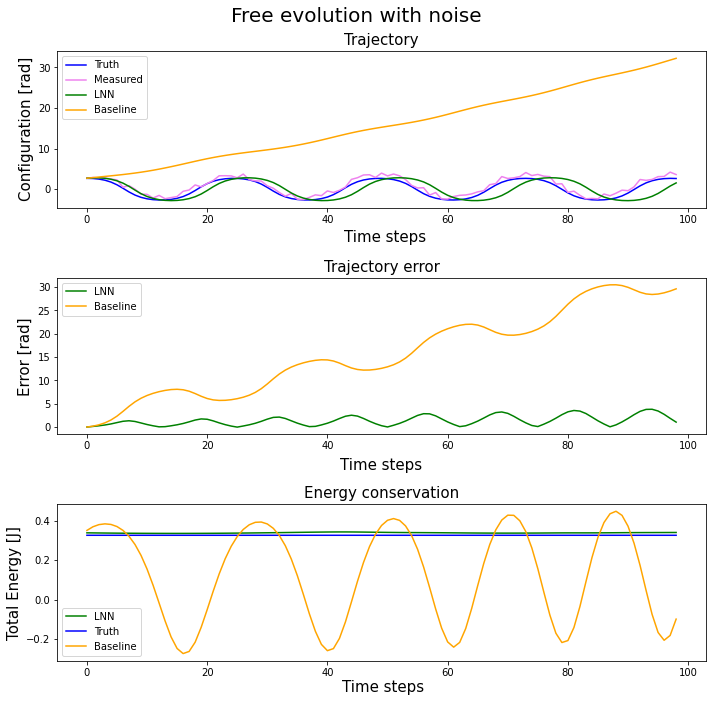
\includegraphics[width=6.5cm ]{img/final_results/rigid/150deg_05rads/rigid_baseline_noise_150_05.png} }}
    \caption{\textit{Simulation 3}. Graphs of the trajectory, error, and energy conservation for the NN baseline and LNN. In this case, the introduction of noise leads to difficulties for both architectures..}
    \label{fig:rigid_150degrees_05rads}
\end{figure}

What we have seen in previous simulations is repeated now. Especially for the noiseless case, we get very similar results to \textit{Simulation 1}, with the NN baseline trajectory not good, and the LNN trajectory starting to lag after a few time steps

\begin{table}
    \centering
    \caption{\textit{Simulation 3.} LNN and baseline NN RMSE on the whole desired trajectory for initial conditions $q(0)=2.66\, rad$, $\dot{q}(0)=0.5\, \frac{rad}{s}$}
    \begin{tabular}{P{2.5cm}P{2.5cm}P{2.5cm}} 
    \hline\hline
    \textbf{Network} & \textbf{No noise} & \textbf{Noise} \\ 
    \hline
     Baseline NN & $2.5636\, [rad]$ & $18.1152\, [rad]$\\
    \hline
     LNN & $0.5096\, [rad]$& $1.7531\, [rad]$\\
    \hline\hline
    \end{tabular}
    \label{tab:rigid_rmse_3}    
\end{table}

In this last simulation, however, both architectures suffer more from the introduction of noise. With the disturbance of the measurement from which to predict trajectories, the NN baseline again exhibits abnormal behavior as in \textit{Simulation 2}. The LNN is also relatively more distressed than in previous cases. It can be seen from the graph in Figure \ref{fig:rigid_150degrees_05rads}, how from the very beginning of the trajectory, the prediction of the LNN turns out to lag behind the ground truth, with this effect increasing with time. This fact is also confirmed by the values in table \ref{tab:rigid_rmse_3}. We also note that the total energy of the LNN, compared to the previous simulations, undergoes a slight deviation from the actual total energy. However, overall the LNN again maintains better behavior than the baseline NN.



%---> Networks setup
\subsection{Elastic case}
In the elastic context, the link parameters of the 1R robot remain unchanged, but the motor and the elastic characteristics should be added to the discussion. Thus, the following additional parameters should be considered for the elastic robot:

\begin{itemize}
    \item Motor height ($h_m$).
    \item Motor base radius ($r_m$).
    \item Motor mass ($m_m$).
    \item Reduction ratio ($n_r$).
    \item Motor inertia ($I_m$).
    \item Stiffness constant ($I_m$).
\end{itemize}

As for the motor, we will make the following assumptions:
\begin{itemize}
    \item It is a low steel cylinder.
    \item Its mass is uniformly distributed.
    \item Its density is $D_{steel}=7850 \frac{kg}{m^3}$.
    \item Its inertia is mainly given by its base radius $r_m$.
\end{itemize} 

By specializing the formulas in \eqref{eq:cilinder} for this case study, we can derive the parameters of the elastic robot that we will use in subsequent simulations, remembering that we consider the motors after reduction, as expressed in Section \ref{sec:robot}

\begin{table}
\centering
\caption{Elastic robot parameters}
\begin{tabular}{P{4.5cm}P{2.5cm}} 
\hline\hline
 \textbf{Parameter} & \textbf{Measure} \\ 
\hline
 Height & $0.04\, [m]$\\ 
\hline
 Base radius & $0.02\, [m]$\\ 
\hline
 Mass & $0.4\, [kg]$\\ 
\hline
 Reduction ratio & $160$\\
\hline
 Inertia & $0.0128\, [kg\,m^2]$\\
\hline
 Stiffness constant & $50\, [Nm/rad]$\\
\hline\hline
\end{tabular}
\end{table}

The value of the stiffness constant was decided after observing some values in \cite{giusti} and then slightly adapted to the code implemented from \cite{lnncranmer}.

\subsubsection{Network setup}
\label{subsubsec:nn_elastic}
The structural parameters of the networks, in this case, are very similar to those reported in \ref{sub:rig_sims}. However, the case study on which the networks will be tested is a new application, at least for the approach shown in \cite{lnncranmer}. For this reason, the architectures that will be tested will have three different structures, to see how the response of the different complexity of the architectures to the proposed task varies. Specifically, 3 different configurations are proposed

\begin{table}
    \centering
    \caption{NN parameters for elastic robot simulations}
    \begin{tabular}{P{2.5cm}P{2.5cm}P{2.5cm}} 
    \hline\hline
    \textbf{Configuration} & \textbf{Units} & \textbf{Layers} \\ 
    \hline
     A & 300 & 2\\
    \hline
     B & 500 & 4\\
     \hline
     C & 700 & 5\\
    \hline\hline
    \end{tabular}
    \label{tab:elastic_networks}    
\end{table}

All configurations keep Softplus as the trigger function, following what is indicated in \cite{lnncranmer}. Again, the characteristics of network training are the same as those presented in Section \ref{sub:rigid_train}
%---> Rigid Results
\subsubsection{Results - Configuration A}
\begin{figure}
    \centering
    \subfloat[\centering Baseline NN]{{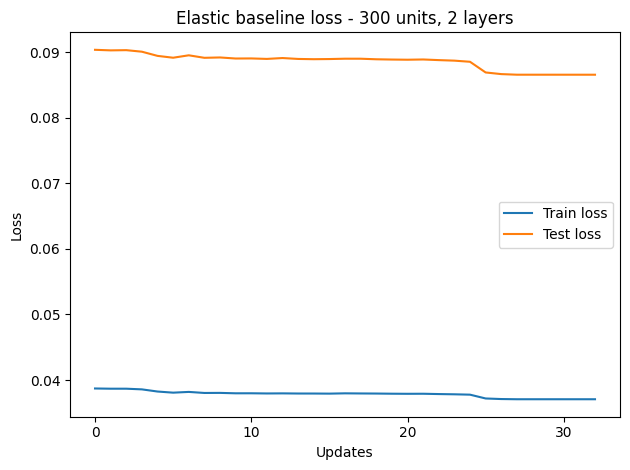
\includegraphics[width=6.5cm]{img/final_results/elastic/300_2/loss/elastic_baseline_loss_300_2.png} }}
    \qquad
    \subfloat[\centering LNN]{{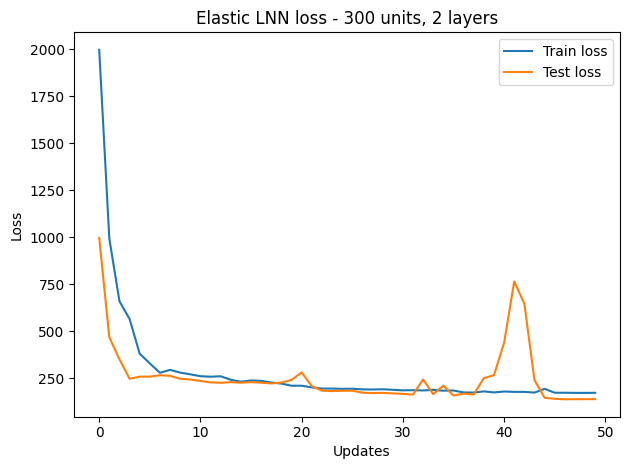
\includegraphics[width=6.5cm]{img/final_results/elastic/300_2/loss/lnn_elastic_loss_300_2.png} }}
    \caption{Test and train losses}
    \label{fig:elastic_losses_300_2}
\end{figure}

Analyzing what the data from the training phase shows us in Figure \ref{fig:elastic_losses_300_2}, we can immediately see problems in the learning phase. The baseline NN loss turns out to drop very slowly, while the LNN loss starts from a high value and, just before the end of the training, has a peak in the test loss. After the training phase, which did not give at all encouraging results, we proceed to test the models on various trajectories, showing the most significant results.\\

\textbf{Simulation 1:} \textbf{Trajectory with $q(0)=2.66\, rad$, $\dot{q}(0)=0.5\, \frac{rad}{s}, \theta(0)=3.06\, rad$, $\dot{\theta}(0)=1\, \frac{rad}{s}$}
In the first elastic case simulation, we analyze the behavior of the two networks when the robot is almost standing vertical

\begin{figure}
    \centering
    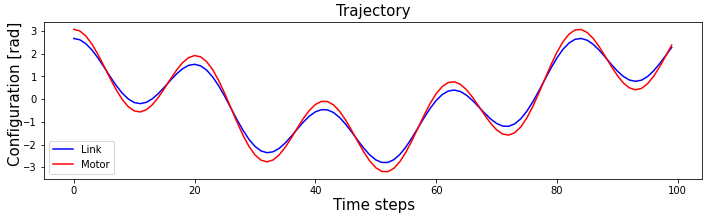
\includegraphics[scale=0.7]{img/final_results/elastic/300_2/150l_175m/traj_150_175.png}
    \caption{\textit{Simulation 1}. The plot of the desired link and motor trajectory for initial conditions $q(0)=2.66\, rad$, $\dot{q}(0)=0.5\, \frac{rad}{s}, \theta(0)=3.06\, rad$, $\dot{\theta}(0)=1\, \frac{rad}{s}$}
    \label{fig:desired_elastic_150_175}
\end{figure}

\begin{figure}
    \centering
    \subfloat[\centering Without noise \label{fig:elastic_300_150_175_a}]{{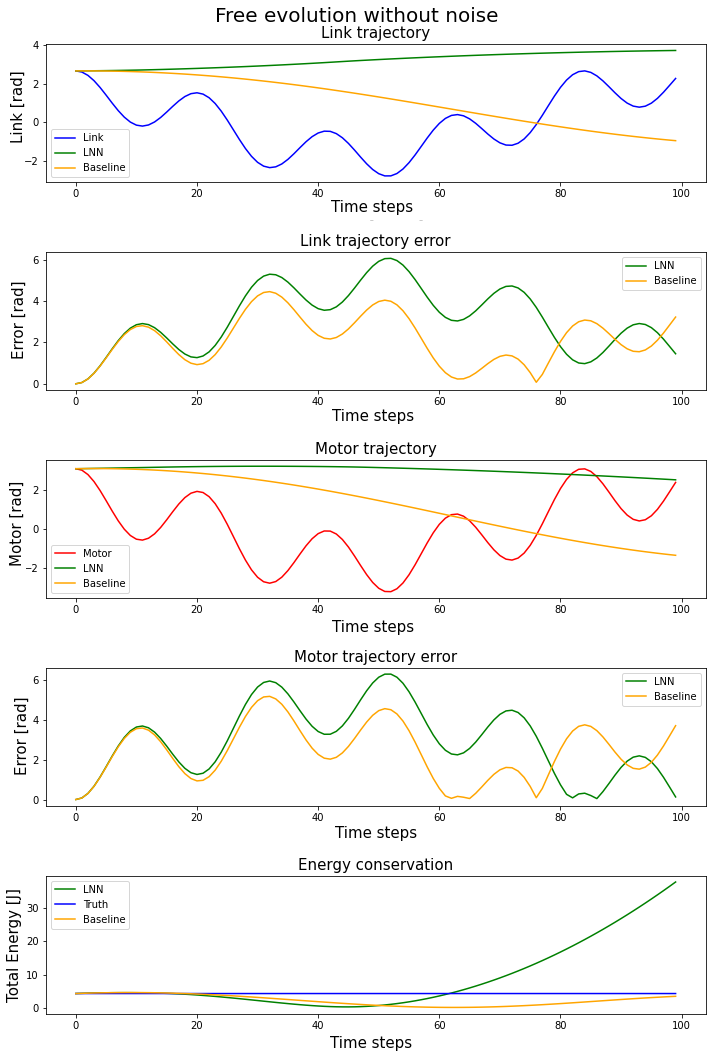
\includegraphics[width=6.5cm]{img/final_results/elastic/300_2/150l_175m/elastic_baseline_freenoise_150_0.5_175_1.png} }}
    \qquad
    \subfloat[\centering With noise \label{fig:elastic_300_150_175_b}]{{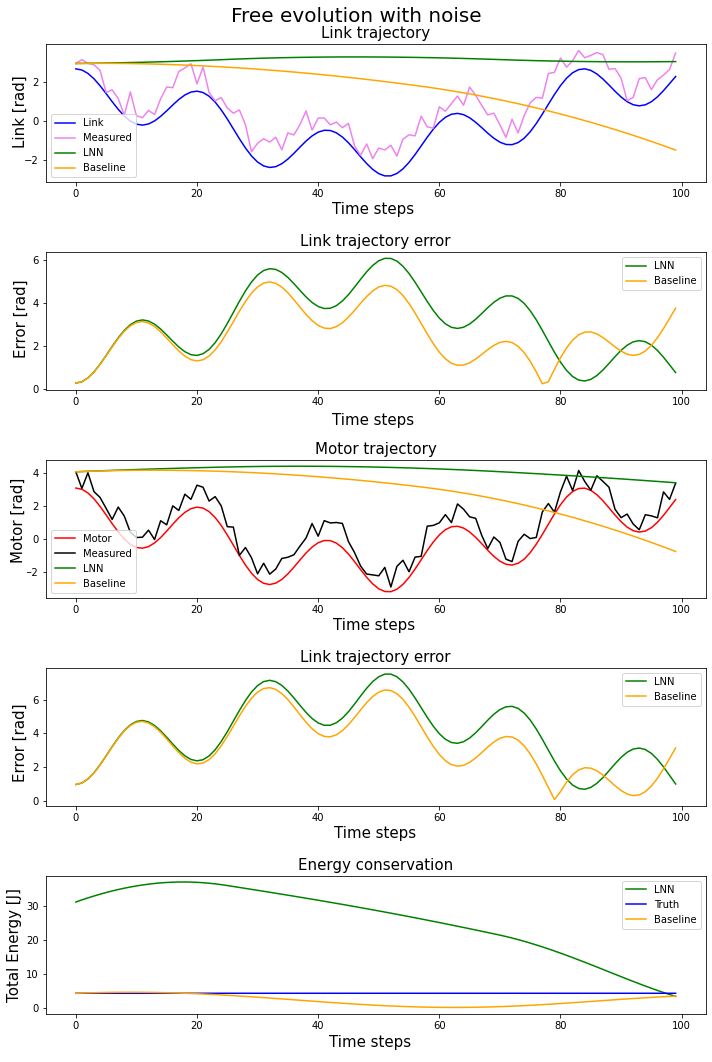
\includegraphics[width=6.5cm ]{img/final_results/elastic/300_2/150l_175m/elastic_baseline_noise_150_0.5_175_1.png} }}
    \caption{\textit{Simulation 1}. Graphs of the trajectory, error, and energy conservation for the NN baseline and LNN. In this first simulation, both networks present enormous difficulties in correctly predicting the desired trajectory, both link, and motor.}
    \label{fig:elastic_300_150_175}
\end{figure}

As well shown by the graphs in figure \ref{fig:elastic_300_150_175}, the first approach to the elastic robot with configuration A does not lead to good results at all. Neither network can correctly predict the evolution of the link and motor trajectories. This appends for both noise and free noise contexts. Moreover, we note how, unlike the rigid case, the LNN in configuration A fails to conserve total energy, reporting strongly abnormal values.

\begin{table}
    \centering
    \caption{\textit{Simulation 1.} LNN and baseline NN RMSE on the whole link desired trajectory for initial conditions $q(0)=2.66\, rad$, $\dot{q}(0)=0.5\, \frac{rad}{s}, \theta(0)=3.06\, rad$, $\dot{\theta}(0)=1\, \frac{rad}{s}$}
    \begin{tabular}{P{2.5cm}P{2.5cm}P{2.5cm}} 
    \hline\hline
    &\textit{Link}&\\
    \hline
    \textbf{Network} & \textbf{No noise} & \textbf{Noise} \\ 
    \hline
     Baseline NN & $2.4337\, [rad]$ & $2.8176\, [rad]$\\
    \hline
     LNN & $3.5242\, [rad]$& $3.4831\, [rad]$\\
    \hline\hline
    \end{tabular}
    \label{tab:elastic_link_rmse_300_1}    
\end{table}

\begin{table}
    \centering
    \caption{\textit{Simulation 1.} LNN and baseline NN RMSE on the whole motor desired trajectory for initial conditions $q(0)=2.66\, rad$, $\dot{q}(0)=0.5\, \frac{rad}{s}, \theta(0)=3.06\, rad$, $\dot{\theta}(0)=1\, \frac{rad}{s}$}
    \begin{tabular}{P{2.5cm}P{2.5cm}P{2.5cm}} 
    \hline\hline
    &\textit{Motor}&\\
    \hline
    \textbf{Network} & \textbf{No noise} & \textbf{Noise} \\ 
    \hline
     Baseline NN & $2.7626\, [rad]$ & $3.8201\, [rad]$\\
    \hline
     LNN & $3.4796\, [rad]$& $4.4901\, [rad]$\\
    \hline\hline
    \end{tabular}
    \label{tab:elastic_motor_rmse_300_1}    
\end{table}

Looking at the RMSE results shown in the tables \ref{tab:elastic_link_rmse_300_1} and \ref{tab:elastic_motor_rmse_300_1}, paradoxically in such wrong results, the NN baseline achieves values that are better in comparisons with those obtained by LNN.\\

\textbf{Simulation 2:} \textbf{Trajectory with $q(0)=1.33\, rad$, $\dot{q}(0)=1\, \frac{rad}{s}, \theta(0)=1.51\, rad$, $\dot{\theta}(0)=0.5\, \frac{rad}{s}$}
In this second simulation, we try lowering the starting position of the robot

\begin{figure}
    \centering
    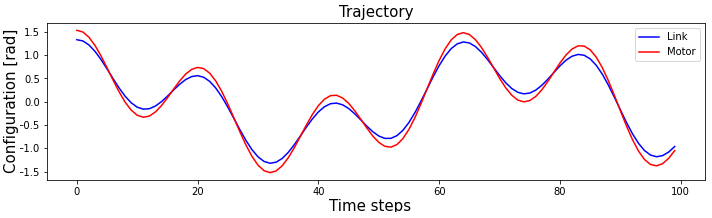
\includegraphics[scale=0.7]{img/final_results/elastic/300_2/76l_87m/traj_76_87.png}
    \caption{\textit{Simulation 1}. The plot of the desired link and motor trajectory for initial conditions $q(0)=1.33\, rad$, $\dot{q}(0)=1\, \frac{rad}{s}, \theta(0)=1.51\, rad$, $\dot{\theta}(0)=0.5\, \frac{rad}{s}$}
    \label{fig:desired_elastic_76_87}
\end{figure}

\begin{figure}
    \centering
    \subfloat[\centering Without noise \label{fig:elastic_300_76_87_a}]{{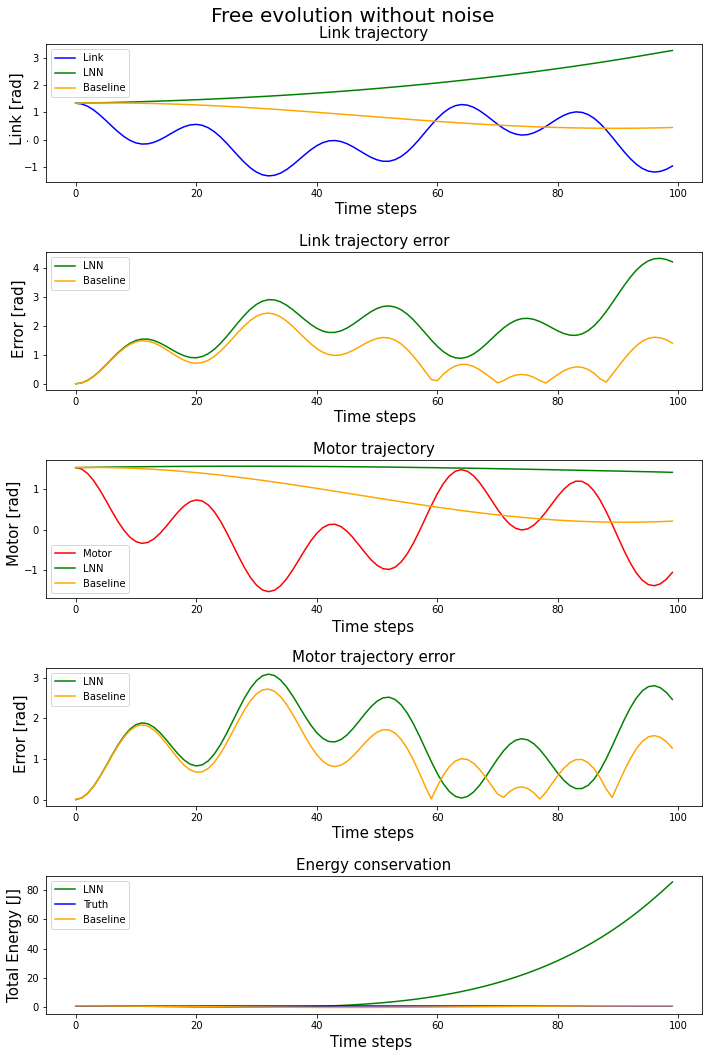
\includegraphics[width=6.5cm]{img/final_results/elastic/300_2/76l_87m/elastic_baseline_freenoise_76_2_87_0.5.png} }}
    \qquad
    \subfloat[\centering With noise \label{fig:elastic_300_76_87_b}]{{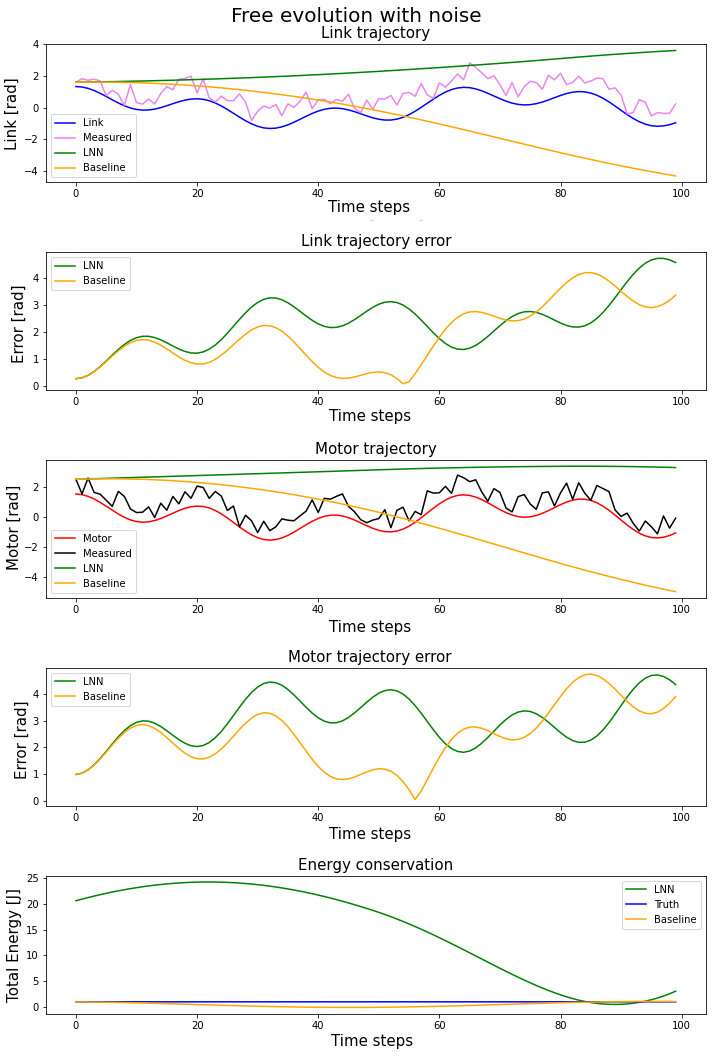
\includegraphics[width=6.5cm ]{img/final_results/elastic/300_2/76l_87m/elastic_baseline_noise_76_2_87_0.5.png.png} }}
    \caption{\textit{Simulation 2}. Graphs of the trajectory, error, and energy conservation for the NN baseline and LNN. The second simulation on a different type of trajectory brings no improvement in the overall context, suggesting that the complexity of the networks is perhaps too low to generalize the problem.}
    \label{fig:elastic_300_76_87}
\end{figure}

The second simulation on a different type of trajectory brings no improvement in the overall context. Indeed, from the point of view of energy conservation, LNN returns even worse results. With the introduction of noise, the quality of the results does not change. 

\begin{table}
    \centering
    \caption{\textit{Simulation 2.} LNN and baseline NN RMSE on the whole link desired trajectory for initial conditions $q(0)=1.33\, rad$, $\dot{q}(0)=1\, \frac{rad}{s}, \theta(0)=1.51\, rad$, $\dot{\theta}(0)=0.5\, \frac{rad}{s}$}
    \begin{tabular}{P{2.5cm}P{2.5cm}P{2.5cm}} 
    \hline\hline
    &\textit{Link}&\\
    \hline
    \textbf{Network} & \textbf{No noise} & \textbf{Noise} \\ 
    \hline
     Baseline NN & $1.1707\, [rad]$ & $2.2049\, [rad]$\\
    \hline
     LNN & $2.1816\, [rad]$& $2.5608\, [rad]$\\
    \hline\hline
    \end{tabular}
    \label{tab:elastic_link_rmse_300_2}    
\end{table}

\begin{table}
    \centering
    \caption{\textit{Simulation 2.} LNN and baseline NN RMSE on the whole motor desired trajectory for initial conditions $q(0)=1.33\, rad$, $\dot{q}(0)=1\, \frac{rad}{s}, \theta(0)=1.51\, rad$, $\dot{\theta}(0)=0.5\, \frac{rad}{s}$}
    \begin{tabular}{P{2.5cm}P{2.5cm}P{2.5cm}} 
    \hline\hline
    &\textit{Motor}&\\
    \hline
    \textbf{Network} & \textbf{No noise} & \textbf{Noise} \\ 
    \hline
     Baseline NN & $1.2734\, [rad]$ & $2.6318\, [rad]$\\
    \hline
     LNN & $1.7103\, [rad]$& $3.1560\, [rad]$\\
    \hline\hline
    \end{tabular}
    \label{tab:elastic_motor_rmse_300_2}    
\end{table}

From the RMSE tables, the values are slightly better than in the previous simulation, but still not sufficient. Moreover, again from the tables \ref{tab:elastic_link_rmse_300_2} and \ref{tab:elastic_motor_rmse_300_2}, we can see how the introduction of noise discretely increases the error. 

These first two simulations on the elastic case show the difficulty of the two types of networks, but analyzing the results obtained suggests, most likely, that the complexity of the networks is perhaps too low to generalize the problem, as from the various indices available, we can see that both the baseline NN and LNN fail to capture important features from the data.\\

\subsubsection{Results - Configuration B}
\begin{figure}
    \centering
    \subfloat[\centering Baseline NN]{{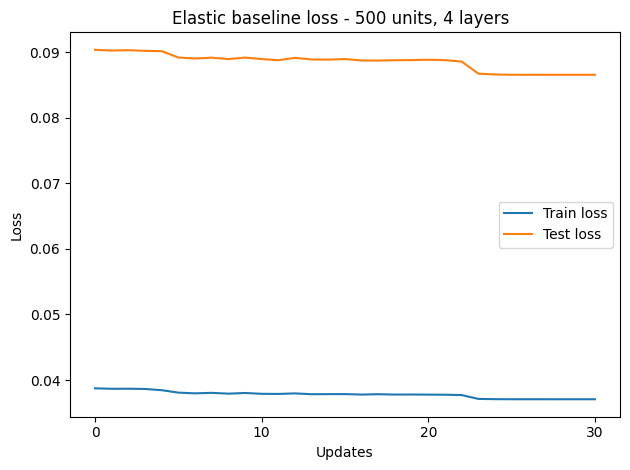
\includegraphics[width=6.5cm]{img/final_results/elastic/500_4/loss/elastic_baseline_loss_500_4.png} }}
    \qquad
    \subfloat[\centering LNN]{{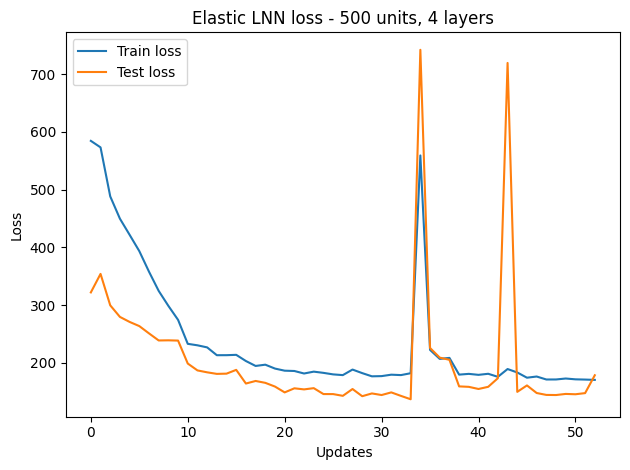
\includegraphics[width=6.5cm]{img/final_results/elastic/500_4/loss/lnn_elastic_loss_500_4.png} }}
    \caption{Test and train losses}
    \label{fig:elastic_losses_500_4}
\end{figure}

The increase in network complexity brings the first changes already during the network training phase, as we can see in figure \ref{fig:elastic_losses_500_4}. Although the baseline NN maintains very similar learning compared to the configuration of the previous case, with a loss that hardly ever decreases, the LNN undergoes important changes. Both the initial and final losses are better than the previous case, although they still maintain a high value. Another sign that should not be underestimated is the presence of LNN loss peaks toward the end of the training session. To carefully evaluate the changes that have occurred, we set the simulations to the same trajectories as in the previous case.\\

\textbf{Simulation 3:} \textbf{Trajectory with $q(0)=2.66\, rad$, $\dot{q}(0)=0.5\, \frac{rad}{s}, \theta(0)=3.06\, rad$, $\dot{\theta}(0)=1\, \frac{rad}{s}$}
The trajectory is the same as shown in figure \ref{fig:desired_elastic_150_175}.

\begin{figure}
    \centering
    \subfloat[\centering Without noise \label{fig:elastic_500_150_175_a}]{{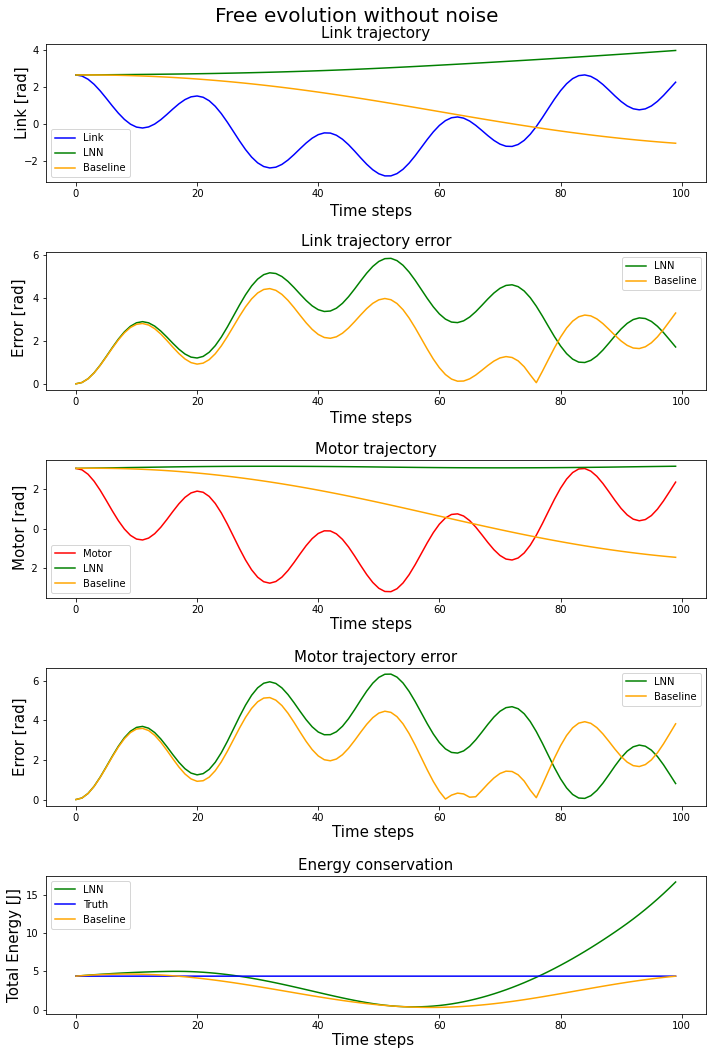
\includegraphics[width=6.5cm]{img/final_results/elastic/500_4/150_175/elastic_baseline_freenoise_150_0.5_175_1.png} }}
    \qquad
    \subfloat[\centering With noise \label{fig:elastic_500_150_175_b}]{{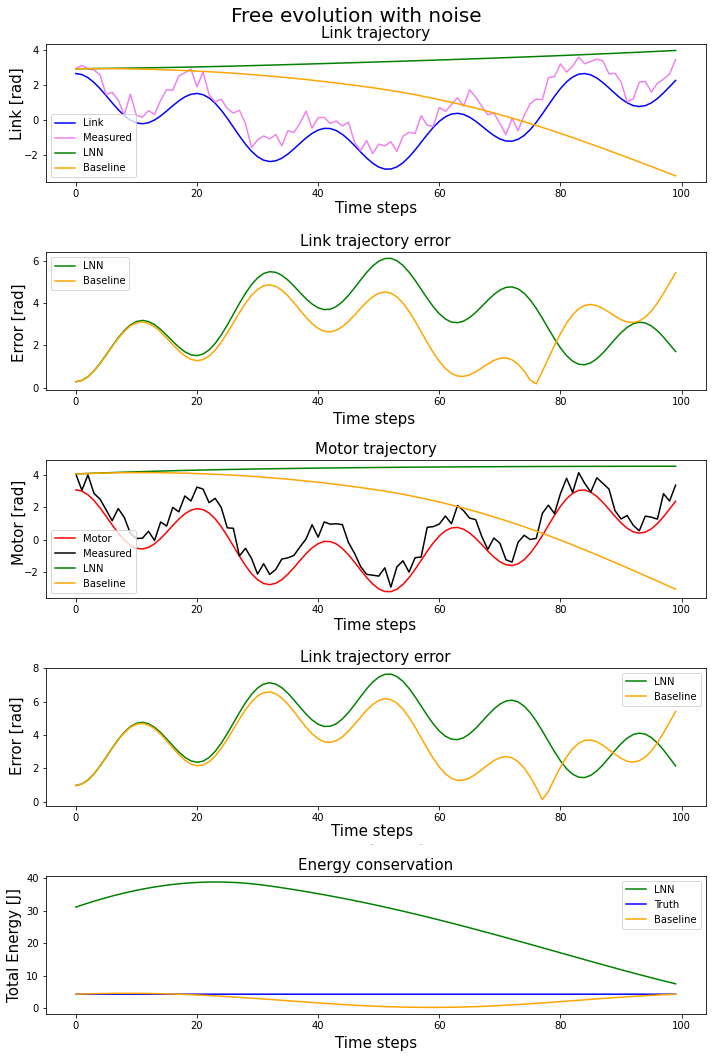
\includegraphics[width=6.5cm ]{img/final_results/elastic/500_4/150_175/elastic_baseline_noise_150_0.5_175_1.png} }}
    \caption{\textit{Simulation 3}. Graphs of the trajectory, error, and energy conservation for the NN baseline and LNN. Despite the increased complexity of the networks, the changes that have taken place are still too weak to speak of good results.}
    \label{fig:elastic_500_150_175}
\end{figure}

Looking at the graphs of \ref{fig:elastic_500_150_175}, the general situation is almost unchanged compared to the previous configuration, although the LNN seems to have had a change in its performance compared to the NN baseline, which remains more or less the same. The error intensity of the LNN is slightly lower, for both the link and motor trajectories. This trend seems to be confirmed even when noise is introduced, naturally without any noticeable results.\\

\begin{table}
    \centering
    \caption{\textit{Simulation 3.} LNN and baseline NN RMSE on the whole link desired trajectory for initial conditions $q(0)=2.66\, rad$, $\dot{q}(0)=0.5\, \frac{rad}{s}, \theta(0)=3.06\, rad$, $\dot{\theta}(0)=1\, \frac{rad}{s}$}
    \begin{tabular}{P{2.5cm}P{2.5cm}P{2.5cm}} 
    \hline\hline
    &\textit{Link}&\\
    \hline
    \textbf{Network} & \textbf{No noise} & \textbf{Noise} \\ 
    \hline
     Baseline NN & $2.4253\, [rad]$ & $2.9910\, [rad]$\\
    \hline
     LNN & $3.4193\, [rad]$& $3.6460\, [rad]$\\
    \hline\hline
    \end{tabular}
    \label{tab:elastic_link_rmse_500_1}    
\end{table}

\begin{table}
    \centering
    \caption{\textit{Simulation 3.} LNN and baseline NN RMSE on the whole motor desired trajectory for initial conditions $q(0)=2.66\, rad$, $\dot{q}(0)=0.5\, \frac{rad}{s}, \theta(0)=3.06\, rad$, $\dot{\theta}(0)=1\, \frac{rad}{s}$}
    \begin{tabular}{P{2.5cm}P{2.5cm}P{2.5cm}} 
    \hline\hline
    &\textit{Motor}&\\
    \hline
    \textbf{Network} & \textbf{No noise} & \textbf{Noise} \\ 
    \hline
     Baseline NN & $2.7547\, [rad]$ & $3.8176\, [rad]$\\
    \hline
     LNN & $3.4556\, [rad]$& $4.3988\, [rad]$\\
    \hline\hline
    \end{tabular}
    \label{tab:elastic_motor_rmse_500_1}    
\end{table}

Even from the RMSE values, LNN seems to bring very slight signs of change. Comparing these results with those of the previous configuration table, a slight improvement in the statistics can be seen. However, once again, the introduction of noise worsens these values, showing the low robustness of this architecture. The NN baseline, on the other hand, keeps them relatively unchanged.\\

\textbf{Simulation 4:} \textbf{Trajectory with $q(0)=1.33\, rad$, $\dot{q}(0)=1\, \frac{rad}{s}, \theta(0)=1.51\, rad$, $\dot{\theta}(0)=0.5\, \frac{rad}{s}$}
Also, in this case, the trajectory is the same as shown in figure \ref{fig:desired_elastic_76_87}.

\begin{figure}
    \centering
    \subfloat[\centering Without noise \label{fig:elastic_500_76_87_a}]{{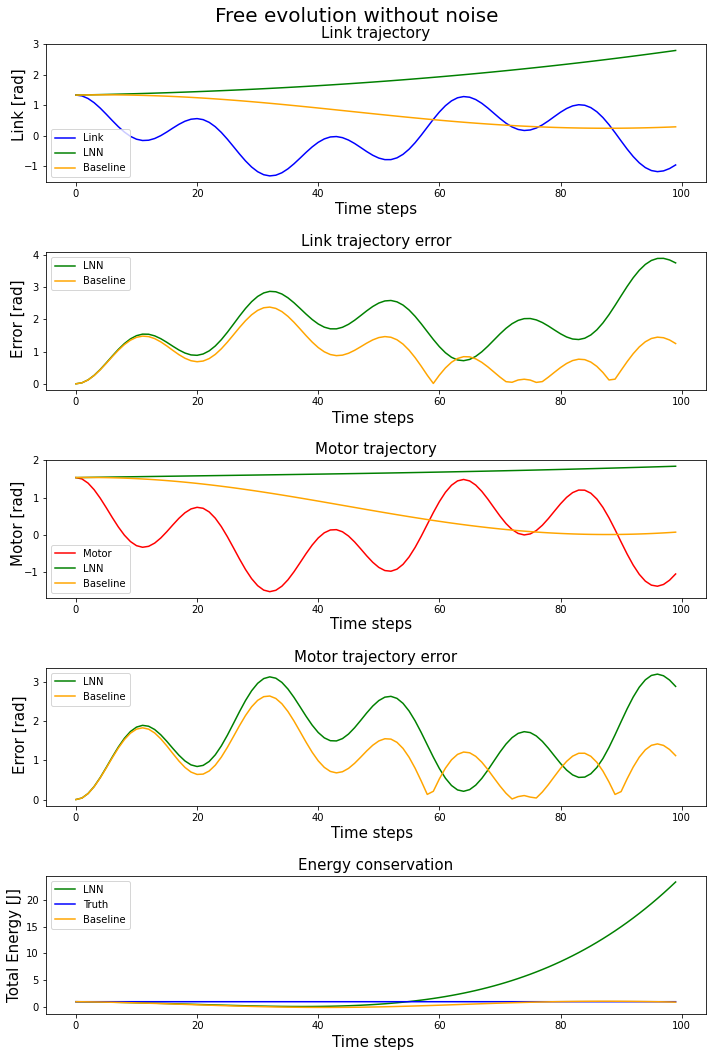
\includegraphics[width=6.5cm]{img/final_results/elastic/500_4/76degreeslink_87degreesmotor/elastic_baseline_freenoise_76_2_87_0.5.png} }}
    \qquad
    \subfloat[\centering With noise \label{fig:elastic_500_76_87_b}]{{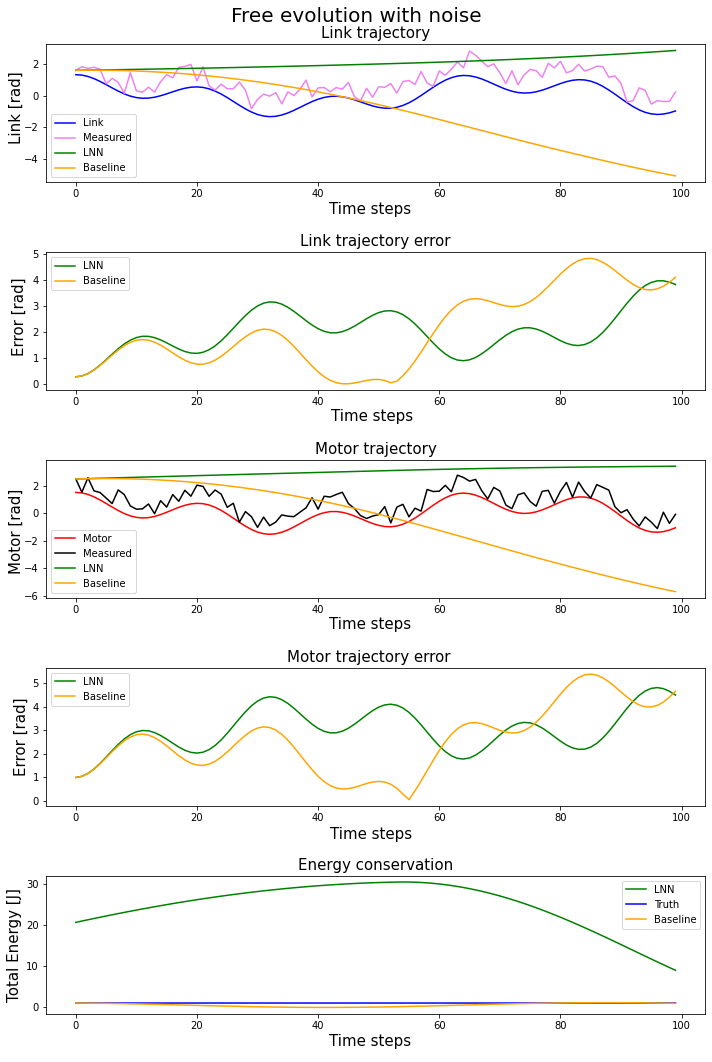
\includegraphics[width=6.5cm ]{img/final_results/elastic/500_4/76degreeslink_87degreesmotor/elastic_baseline_noise_76_2_87_0.5.png.png} }}
    \caption{\textit{Simulation 4}. Graphs of the trajectory, error, and energy conservation for the NN baseline and LNN. Again, we see a very similar situation to the simulation before this one the results show a trend towards improvement, even if minimal.}
    \label{fig:elastic_500_76_87}
\end{figure}

So far, from the results shown in \ref{fig:elastic_500_76_87}, we can begin to confirm the insights gained from the previous simulation. The results are of course not good, but the error values are dropping slightly as the complexity of the networks increases. It should still be noted that LNN still fails to generalize the conservation of total energy.

\begin{table}
    \centering
    \caption{\textit{Simulation 4.} LNN and baseline NN RMSE on the whole link desired trajectory for initial conditions $q(0)=1.33\, rad$, $\dot{q}(0)=1\, \frac{rad}{s}, \theta(0)=1.51\, rad$, $\dot{\theta}(0)=0.5\, \frac{rad}{s}$}
    \begin{tabular}{P{2.5cm}P{2.5cm}P{2.5cm}} 
    \hline\hline
    &\textit{Link}&\\
    \hline
    \textbf{Network} & \textbf{No noise} & \textbf{Noise} \\ 
    \hline
     Baseline NN & $1.1247\, [rad]$ & $2.5380\, [rad]$\\
    \hline
     LNN & $2.0212\, [rad]$& $2.1989\, [rad]$\\
    \hline\hline
    \end{tabular}
    \label{tab:elastic_link_rmse_500_2}    
\end{table}

\begin{table}
    \centering
    \caption{\textit{Simulation 4.} LNN and baseline NN RMSE on the whole motor desired trajectory for initial conditions $q(0)=1.33\, rad$, $\dot{q}(0)=1\, \frac{rad}{s}, \theta(0)=1.51\, rad$, $\dot{\theta}(0)=0.5\, \frac{rad}{s}$}
    \begin{tabular}{P{2.5cm}P{2.5cm}P{2.5cm}} 
    \hline\hline
    &\textit{Motor}&\\
    \hline
    \textbf{Network} & \textbf{No noise} & \textbf{Noise} \\ 
    \hline
     Baseline NN & $1.2359\, [rad]$ & $2.9295\, [rad]$\\
    \hline
     LNN & $1.6357\, [rad]$& $3.1532\, [rad]$\\
    \hline\hline
    \end{tabular}
    \label{tab:elastic_motor_rmse_500_2}    
\end{table}

What was presented in the previous paragraph is underlined by the values of \ref{tab:elastic_link_rmse_500_2} and \ref{tab:elastic_motor_rmse_500_2}. As far as LNN is concerned, however, it should be noted that these changes are on the order of tens of units for the RMSEE values, which is still too small an improvement. On the other hand, the NN baseline oscillates at values very similar to previous applications.\\

At the end of this fourth simulation, it could be seen that the increase in complexity has somewhat modified the performance of the networks, positively, especially the LNN, which seems to have benefited the most from the changes. However, these improvements are still very low, so in the last two simulations, we propose we will try to increase the width and depth of the networks even more.\\

\subsubsection{Results - Configuration C}
\begin{figure}
    \centering
    \subfloat[\centering Baseline NN]{{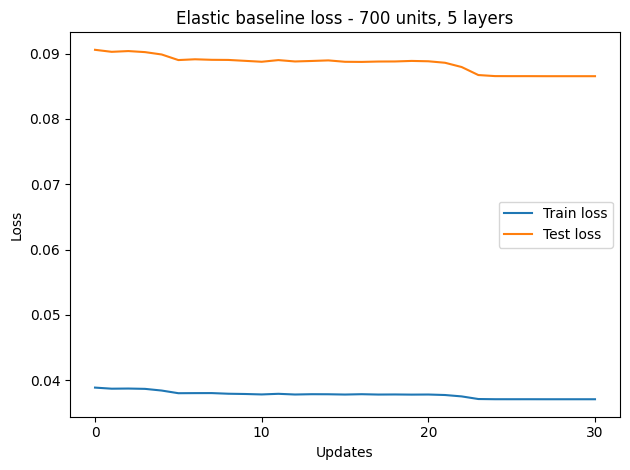
\includegraphics[width=6.5cm]{img/final_results/elastic/700_5/loss/elastic_baseline_loss_700_5.png} }}
    \qquad
    \subfloat[\centering LNN]{{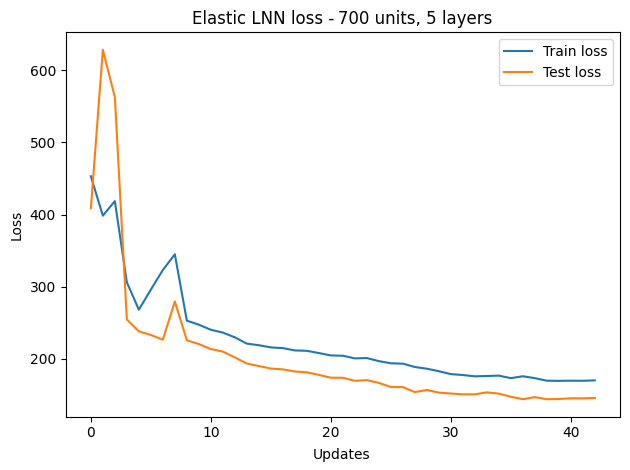
\includegraphics[width=6.5cm]{img/final_results/elastic/700_5/loss/lnn_elastic_loss_700_5.png} }}
    \caption{Test and train losses}
    \label{fig:elastic_losses_700_5}
\end{figure}

The further step of increasing the complexity of the networks brings back interesting results in the LNN train. In fact, from the figure \ref{fig:elastic_losses_700_5}, following some initial oscillations of the loss, which we can define as canonical in a neural network training context, for the first time since the beginning of the simulations on the elastic case, the loss falls gradually and without peaks, although maintaining a high final value. Overall, this is certainly a positive indicator in the context of the NN training. The NN baseline, on the other hand, as it had begun to show in the previous setup, maintains its loss trend without any great drops. One thing to note is that, for the LNN in particular, the training time has increased dramatically with the new configuration imposed on the networks. Also in these simulations, to maintain a term of comparison, we will test the trained networks on the trajectories already presented.\\

\textbf{Simulation 5:} \textbf{Trajectory with $q(0)=2.66\, rad$, $\dot{q}(0)=0.5\, \frac{rad}{s}, \theta(0)=3.06\, rad$, $\dot{\theta}(0)=1\, \frac{rad}{s}$}
The trajectory for this simulation is also similar to that in figure \ref{fig:desired_elastic_150_175}.

\begin{figure}
    \centering
    \subfloat[\centering Without noise \label{fig:elastic_700_150_175_a}]{{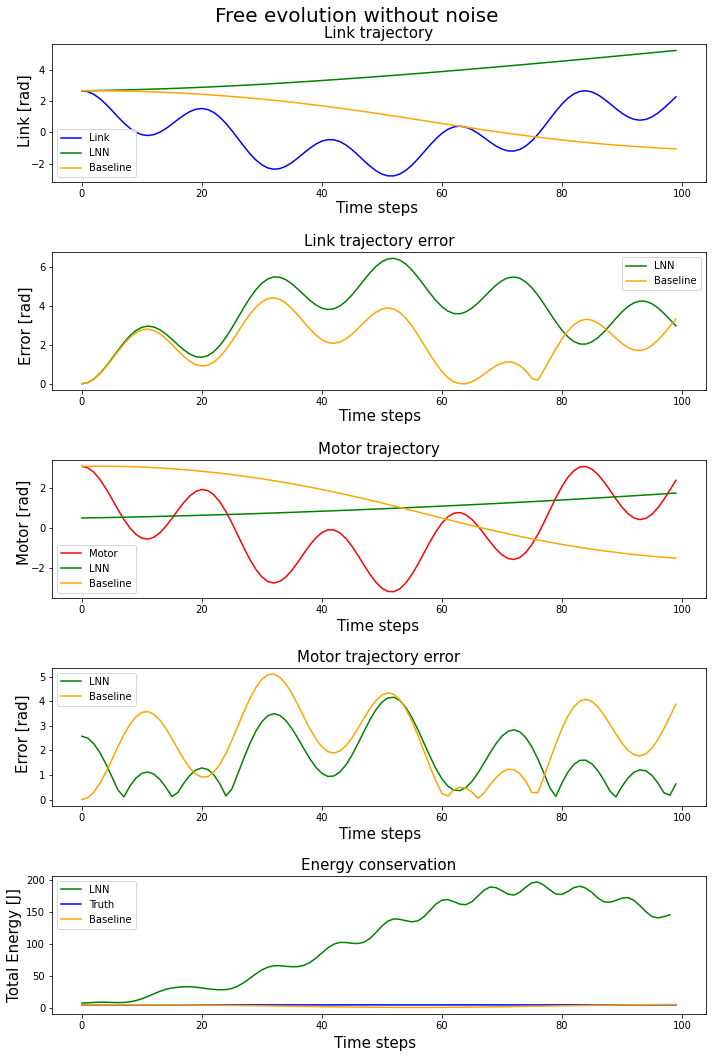
\includegraphics[width=6.5cm]{img/final_results/elastic/700_5/150_175/elastic_baseline_freenoise_150_0.5_76_1.png} }}
    \qquad
    \subfloat[\centering With noise \label{fig:elastic_700_150_175_b}]{{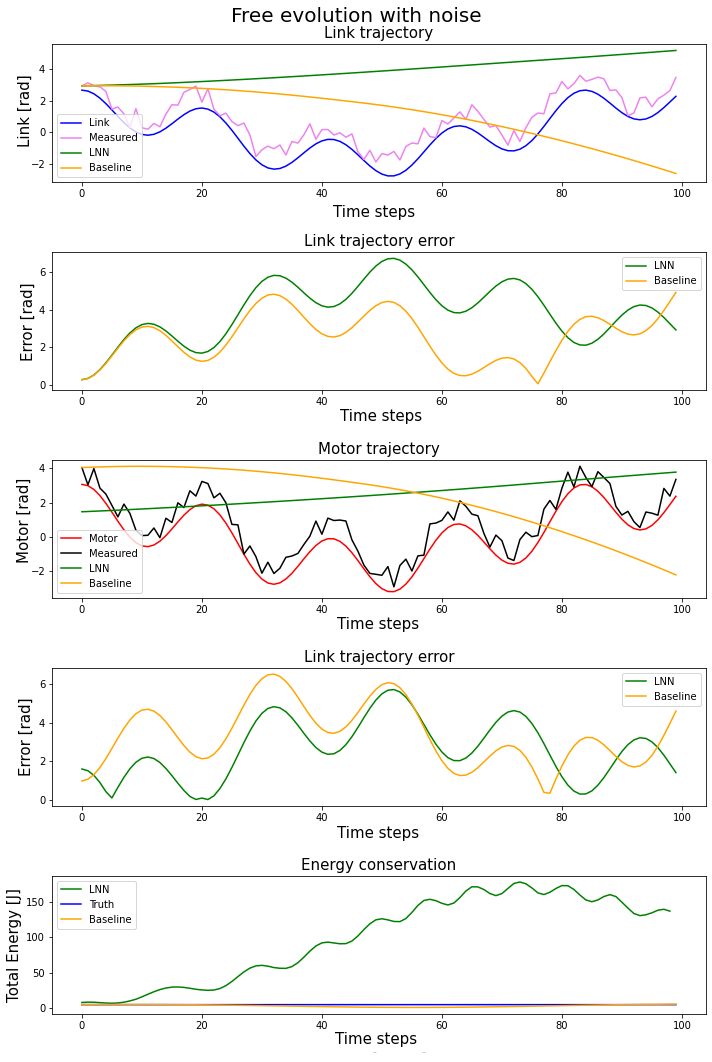
\includegraphics[width=6.5cm ]{img/final_results/elastic/700_5/150_175/elastic_baseline_noise_150_0.5_76_1.png} }}
    \caption{\textit{Simulation 5}. Graphs of the trajectory, error, and energy conservation for the NN baseline and LNN. The slight effects of increased network complexity continue, in particular for the first time the total energy of the LNN does not diverge.}
    \label{fig:elastic_700_150_175}
\end{figure}

The analysis of the training data only partially confirms the intuition of the improved situation. Once again, neither architecture was able to correctly predict the trajectory of the link and motor. However, for the first time since the elastic case simulations began, the total energy of the LNN does not diverge, remaining limited, albeit at an abnormal value compared to ground truth. The situation just described is also confirmed in the case of the introduction of noise.

\begin{table}
    \centering
    \caption{\textit{Simulation 5.} LNN and baseline NN RMSE on the whole link desired trajectory for initial conditions $q(0)=2.66\, rad$, $\dot{q}(0)=0.5\, \frac{rad}{s}, \theta(0)=3.06\, rad$, $\dot{\theta}(0)=1\, \frac{rad}{s}$}
    \begin{tabular}{P{2.5cm}P{2.5cm}P{2.5cm}} 
    \hline\hline
    &\textit{Link}&\\
    \hline
    \textbf{Network} & \textbf{No noise} & \textbf{Noise} \\ 
    \hline
     Baseline NN & $2.4173\, [rad]$ & $2.8553\, [rad]$\\
    \hline
     LNN & $3.0199\, [rad]$& $3.1879\, [rad]$\\
    \hline\hline
    \end{tabular}
    \label{tab:elastic_link_rmse_700_1}    
\end{table}

\begin{table}
    \centering
    \caption{\textit{Simulation 4.} LNN and baseline NN RMSE on the whole motor desired trajectory for initial conditions $q(0)=2.66\, rad$, $\dot{q}(0)=0.5\, \frac{rad}{s}, \theta(0)=3.06\, rad$, $\dot{\theta}(0)=1\, \frac{rad}{s}$}
    \begin{tabular}{P{2.5cm}P{2.5cm}P{2.5cm}} 
    \hline\hline
    &\textit{Motor}&\\
    \hline
    \textbf{Network} & \textbf{No noise} & \textbf{Noise} \\ 
    \hline
     Baseline NN & $2.7524\, [rad]$ & $3.6792\, [rad]$\\
    \hline
     LNN & $1.9237\, [rad]$& $3.0289\, [rad]$\\
    \hline\hline
    \end{tabular}
    \label{tab:elastic_motor_rmse_700_1}    
\end{table}

As far as the RMSE values are concerned, the slow decrease of this type of index by LNN continues. It once again decreases by a few tenths of a value. In particular, however, we can at this point definitively confirm the very low robustness of the LNN model for the elastic case in the face of signals with noise. We note above all how in \ref{tab:elastic_motor_rmse_700_1} the corresponding RMSE value increases considerably in correspondence with noise. Moreover, as we expected, the NN baseline remains, in general, in the range of values of the previous simulations.\\

\textbf{Simulation 6:} \textbf{Trajectory with $q(0)=1.33\, rad$, $\dot{q}(0)=1\, \frac{rad}{s}, \theta(0)=1.51\, rad$, $\dot{\theta}(0)=0.5\, \frac{rad}{s}$}
Finally, this trajectory is also the same as in the figure \ref{fig:desired_elastic_76_87}.

\begin{figure}
    \centering
    \subfloat[\centering Without noise \label{fig:elastic_700_76_87_a}]{{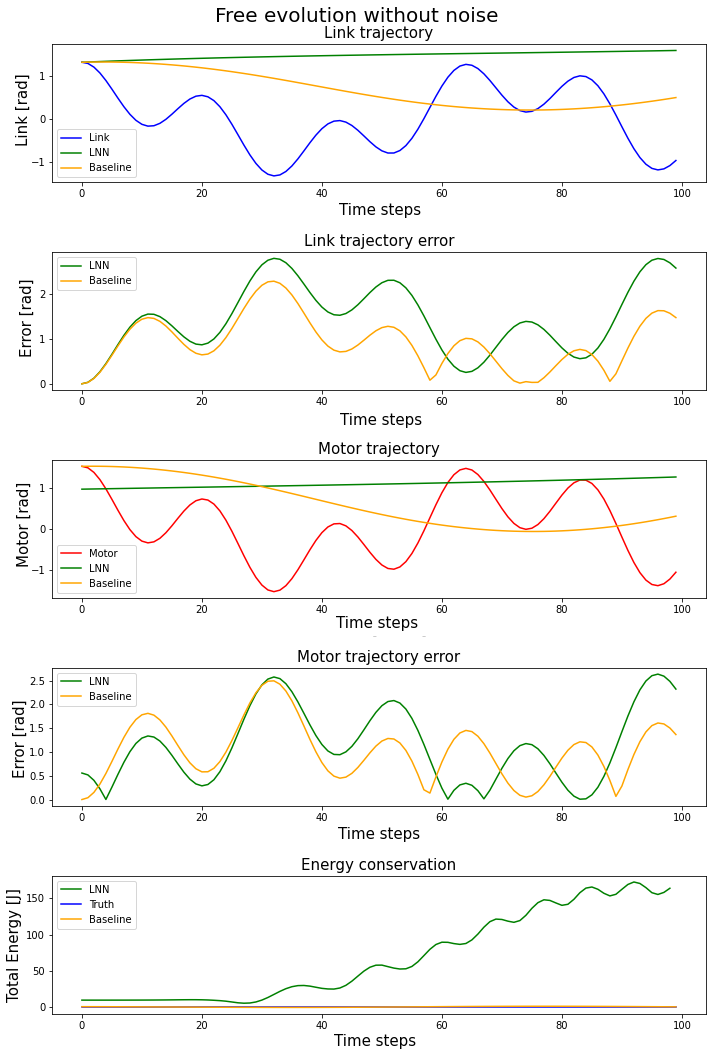
\includegraphics[width=6.5cm]{img/final_results/elastic/700_5/76degreeslink_87degreesmotor/elastic_baseline_freenoise_76_2_87_0.5.png} }}
    \qquad
    \subfloat[\centering With noise \label{fig:elastic_700_76_87_b}]{{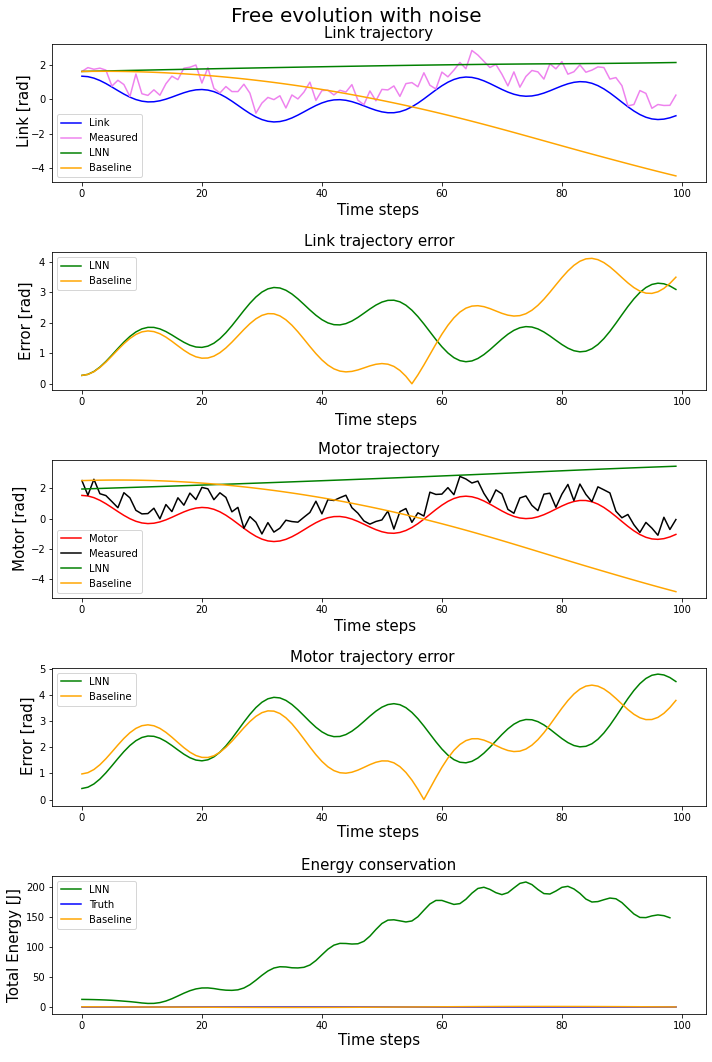
\includegraphics[width=6.5cm ]{img/final_results/elastic/700_5/76degreeslink_87degreesmotor/elastic_baseline_noise_76_2_87_0.5.png.png} }}
    \caption{\textit{Simulation 6}. Graphs of the trajectory, error, and energy conservation for the NN baseline and LNN. The trend of improvements remains very similar to the previous case. Energy conservation by LNN also changes.}
    \label{fig:elastic_700_76_87}
\end{figure}

In this other type of trajectory, we see results in agreement with what has been achieved so far with this configuration of networks. Unfortunately, it must be emphasized that for the umpteenth time in the elastic case, both the LNN and the baseline NN fail to correctly predict the trajectory of the link and the motor, even partially. The major change, as in the previous trajectory, seems to be in the conservation of total energy by the LNN, which seems to be settling without diverging.

\begin{table}
    \centering
    \caption{\textit{Simulation 6.} LNN and baseline NN RMSE on the whole link desired trajectory for initial conditions $q(0)=1.33\, rad$, $\dot{q}(0)=1\, \frac{rad}{s}, \theta(0)=1.51\, rad$, $\dot{\theta}(0)=0.5\, \frac{rad}{s}$}
    \begin{tabular}{P{2.5cm}P{2.5cm}P{2.5cm}} 
    \hline\hline
    &\textit{Link}&\\
    \hline
    \textbf{Network} & \textbf{No noise} & \textbf{Noise} \\ 
    \hline
     Baseline NN & $1.1221\, [rad]$ & $2.1565\, [rad]$\\
    \hline
     LNN & $1.6345\, [rad]$& $2.0139\, [rad]$\\
    \hline\hline
    \end{tabular}
    \label{tab:elastic_link_rmse_700_2}    
\end{table}

\begin{table}
    \centering
    \caption{\textit{Simulation 6.} LNN and baseline NN RMSE on the whole motor desired trajectory for initial conditions $q(0)=1.33\, rad$, $\dot{q}(0)=1\, \frac{rad}{s}, \theta(0)=1.51\, rad$, $\dot{\theta}(0)=0.5\, \frac{rad}{s}$}
    \begin{tabular}{P{2.5cm}P{2.5cm}P{2.5cm}} 
    \hline\hline
    &\textit{Motor}&\\
    \hline
    \textbf{Network} & \textbf{No noise} & \textbf{Noise} \\ 
    \hline
     Baseline NN & $1.2009\, [rad]$ & $2.5066\, [rad]$\\
    \hline
     LNN & $1.3689\, [rad]$& $2.8148\, [rad]$\\
    \hline\hline
    \end{tabular}
    \label{tab:elastic_motor_rmse_700_2}    
\end{table}

The trend presented is also confirmed in the RMSEE values of the tables \ref{tab:elastic_link_rmse_700_2} and \ref{tab:elastic_motor_rmse_700_2}. Once again, the improvement in these indices for LNN is in the order of tens of units. This improvement is lost when noise is introduced, although this deterioration is relatively lower than the same value from configurations A and B. From these considerations, we can definitively confirm the weakness against the noise of the LNN applied in the elastic case. Finally, the baseline NN maintains its values in the range of the previous cases.\\

At the end of the simulations of the elastic case, we can see that the intuition of gradually increasing the complexity of the network has paid off somewhat in terms of performance, although the latter remains not at all good in all tests. For the LNN in particular, this increase in complexity induces a very slow decrease in error, suggesting that perhaps a very drastic increase in the complexity of the network would finally lead to satisfactory and sufficient results. However, given the training time of configuration C, our most complex network, this drastic increase in the depth and breadth of the network would have required high computational resources, requiring suitable tools to support very heavy training.\\


%---------------------------------- Conclusions ------------------------------- %
\section{Conclusions}
At the end of this project, we can observe the following concepts. First of all, at least in the rigid case, it is well demonstrated how the identification of the robot's dynamic model is better using the LNN approach, both in terms of trajectory error and energy conservation. Unfortunately, the good results obtained in the rigid case were not confirmed in the elastic case. However, important and interesting information can be extracted from the simulations of this case. It can be seen from the data obtained that as the complexity of the network increases, the outputs of the Lagrangian seem to change slightly for the better. As we can see, the case for configuration C of the LNN is the only one with non-divergent total energy. This leads us to think that by increasing the complexity of the network, in particular its depth and width, even better results could be achieved. Along with this, one could try to increase the number of initial conditions on which the network is trained. However, these two assumptions for improving the network's performance would presuppose high computational resources, so these insights could only be tested in suitable laboratory settings. A final insight that may arise from our study is that the LNN approach proposed in \cite{lnncranmer} bases its experiments on totally unitary configurations, a concept that we rejected in preference to a configuration as close to reality as possible.


%---------------------------------- Bibliography ------------------------------ %
\bibliographystyle{plain} % We choose the "plain" reference style
\bibliography{ref} % Entries are in the refs.bib file

\end{document}
